% Options for packages loaded elsewhere
\PassOptionsToPackage{unicode}{hyperref}
\PassOptionsToPackage{hyphens}{url}
\documentclass[
]{article}
\usepackage{xcolor}
\usepackage[a4paper,left=1.5cm,right=1.5cm,top=1.5cm,bottom=1.5cm]{geometry}
\usepackage{amsmath,amssymb}
\setcounter{secnumdepth}{-\maxdimen} % remove section numbering
\usepackage{iftex}
\ifPDFTeX
  \usepackage[T1]{fontenc}
  \usepackage[utf8]{inputenc}
  \usepackage{textcomp} % provide euro and other symbols
\else % if luatex or xetex
  \usepackage{unicode-math} % this also loads fontspec
  \defaultfontfeatures{Scale=MatchLowercase}
  \defaultfontfeatures[\rmfamily]{Ligatures=TeX,Scale=1}
\fi
\usepackage{lmodern}
\ifPDFTeX\else
  % xetex/luatex font selection
\fi
% Use upquote if available, for straight quotes in verbatim environments
\IfFileExists{upquote.sty}{\usepackage{upquote}}{}
\IfFileExists{microtype.sty}{% use microtype if available
  \usepackage[]{microtype}
  \UseMicrotypeSet[protrusion]{basicmath} % disable protrusion for tt fonts
}{}
\makeatletter
\@ifundefined{KOMAClassName}{% if non-KOMA class
  \IfFileExists{parskip.sty}{%
    \usepackage{parskip}
  }{% else
    \setlength{\parindent}{0pt}
    \setlength{\parskip}{6pt plus 2pt minus 1pt}}
}{% if KOMA class
  \KOMAoptions{parskip=half}}
\makeatother
\usepackage{graphicx}
\makeatletter
\newsavebox\pandoc@box
\newcommand*\pandocbounded[1]{% scales image to fit in text height/width
  \sbox\pandoc@box{#1}%
  \Gscale@div\@tempa{\textheight}{\dimexpr\ht\pandoc@box+\dp\pandoc@box\relax}%
  \Gscale@div\@tempb{\linewidth}{\wd\pandoc@box}%
  \ifdim\@tempb\p@<\@tempa\p@\let\@tempa\@tempb\fi% select the smaller of both
  \ifdim\@tempa\p@<\p@\scalebox{\@tempa}{\usebox\pandoc@box}%
  \else\usebox{\pandoc@box}%
  \fi%
}
% Set default figure placement to htbp
\def\fps@figure{htbp}
\makeatother
\setlength{\emergencystretch}{3em} % prevent overfull lines
\providecommand{\tightlist}{%
  \setlength{\itemsep}{0pt}\setlength{\parskip}{0pt}}
\usepackage[]{natbib}
\bibliographystyle{apalike}
\usepackage{caption}
\usepackage{float}
\usepackage{tabularray}
\usepackage{booktabs}
\usepackage{siunitx}
\usepackage{titlesec}
\UseTblrLibrary{booktabs}
\captionsetup{font=small,labelfont=bf}
\graphicspath{{output/figures/}{output/clusterings/maps/}}
\setlength{\parskip}{0.18em}
\setlength{\parindent}{0pt}
\titlespacing*{\section}{0pt}{0.8ex plus 0.2ex}{0.5ex}
\titlespacing*{\subsection}{0pt}{0.6ex plus 0.2ex}{0.3ex}
\titlespacing*{\paragraph}{0pt}{0.4ex plus 0.1ex}{0.5em}
\usepackage{bookmark}
\IfFileExists{xurl.sty}{\usepackage{xurl}}{} % add URL line breaks if available
\urlstyle{same}
\hypersetup{
  pdftitle={\textbackslash{} Advanced Econometrics II: Non-standard Inference and Simulation},
  pdfauthor={Stephane KWEKE NGAHANE, Yumiao TIAN, Thomas BOMBARDE},
  hidelinks,
  pdfcreator={LaTeX via pandoc}}

\title{\Large \textbf{Fixed-\(G\) Inference with Climate-Based Clusters}\textbackslash{}
\large Advanced Econometrics II: Non-standard Inference and
Simulation\footnote{\url{https://github.com/Thomas-Bombarde/Adv.Metrics-Assignment-2026}}}
\author{Stephane KWEKE NGAHANE, Yumiao TIAN, Thomas BOMBARDE}
\date{}

\begin{document}
\maketitle

\section{Introduction}

\citet{bester_conley_hansen_2011}, hereafter BCH, study inference with
dependent data using cluster covariance estimators. Their contribution
is a fixed-\(G\) theory for settings where observations are divided into
a few large groups. The covariance matrix is estimated from group score
sums, and critical values reflect that only a small number of groups are
available. A central result is that, if \(G\) is fixed and group size
grows, the cluster covariance estimator remains random. For a scalar
coefficient, the BCH statistic is therefore compared with \(t_{G-1}\),
not \(N(0,1)\). The practical requirement is not simply many clusters.
It is large, well-shaped groups whose score sums are approximately
independent.

This report uses that result to ask one empirical question with two
parts: does the number of groups change inference in a spatial
climate-conflict application, and how can groups be chosen when small
spatial units are correlated but the true dependence structure is
unknown? The setting comes from \citet{burke2024}, who study whether
wealth weakens the link between weather shocks and civil conflict in
Africa. Their replication package constructs a spatially disaggregated
panel from Berkeley Earth temperature data, UCDP georeferenced conflict
events, local wealth estimates, and national GDP per capita. We use the
public weather-conflict component of this package. The broader
climate-conflict literature summarized by
\citet{hsiang_burke_miguel_2013} remains useful context, but Burke et
al.~(2024) provide the direct empirical motivation.

The report proceeds in four steps. First, a simulation reproduces the
fixed-\(G\) mechanism: changing \(G\) changes both variance estimation
and the reference distribution. Second, candidate regions are
constructed from temperature-anomaly co-movement using HiClimR
\citep{badr_zaitchik_dezfuli_2015}. The groups are based on treatment
dynamics, not conflict outcomes. Third, a fixed-effects climate-conflict
model is estimated once, and BCH-style inference is recomputed for
\(G=4,8,12,16,20\). Fourth, score independence is compared across
data-driven climate groups, supranational administrative macroregions,
and country clusters.

Section 2 explains why fixed-\(G\) inference differs from normal cluster
inference. Section 3 applies the question to the Burke et
al.~weather-conflict data: it describes the data, constructs the climate
groups, estimates the model, and compares score diagnostics against
administrative groupings. Section 4 states the resulting interpretation
and its limits.

\section{Monte Carlo Simulation for \texorpdfstring{Fixed-\(G\)}{Fixed-G} Cluster Inference}

The notation below is deliberately stylized to isolate the inferential
mechanism in BCH. It defines a spatial lattice in which both the
regressor and the error are locally dependent, estimates OLS under a
true null, and asks what happens when inference is based on a fixed
number \(G\) of large spatial groups. The objects of interest are the
group-level covariance estimator and the studentized coefficient.

Let \(\mathcal S_K=\{1,\ldots,K\}^2\subset\mathbb Z^2\), \(N_K=K^2\),
and \[
d_\infty(s,t)=\max\{|s_1-t_1|,\ |s_2-t_2|\}.
\] On a two-cell padding of \(\mathcal S_K\), let \(u_r\) and \(v_r\) be
independent Gaussian white-noise fields. For \(\gamma\in\{0,0.3,0.6\}\),
define the spatial moving-average fields \[
x_\gamma(s)=\sum_{d_\infty(h,0)\leq 2}\gamma^{d_\infty(h,0)}v_{s+h},
\qquad
\varepsilon_\gamma(s)=\sum_{d_\infty(h,0)\leq 2}\gamma^{d_\infty(h,0)}u_{s+h}.
\] The outcome is \[
y_\gamma(s)=\beta_0x_\gamma(s)+\varepsilon_\gamma(s),\qquad \beta_0=1,
\] so \(H_0:\beta=\beta_0\) is true in every replication. Let \(X_K\)
have row \((1,x_\gamma(s))\), and write the OLS estimator as \[
\widehat\theta_K=(X_K'X_K)^{-1}X_K'Y_K,\qquad
\widehat\theta_K=(\widehat\alpha_K,\widehat\beta_K)'.
\]

Partition \(\mathcal S_K\) into \(G\) equal contiguous blocks. With
\(X_{g,K}\) and \(\widehat e_{g,K}\) denoting observations and residuals
in group \(g\), the cluster covariance estimator is \[
\widehat V_K^{CCE}
=\frac{1}{N_K}\sum_{g=1}^{G}X_{g,K}'\widehat e_{g,K}\widehat e_{g,K}'X_{g,K}.
\] Let \(\widehat Q_K=N_K^{-1}X_K'X_K\), and \(a=(0,1)'\). The raw CCE
statistic is \[
T_K^{CCE}=
\frac{\sqrt{N_K}(a'\widehat\theta_K-\beta_0)}
{\left[a'\widehat Q_K^{-1}\widehat V_K^{CCE}\widehat Q_K^{-1}a\right]^{1/2}},
\] whereas the BCH statistic rescales it as \[
T_K^{BCH}=\sqrt{\frac{G-1}{G}}\,T_K^{CCE}
\quad\text{and is compared with }t_{G-1}.
\]

The interpretation follows the main BCH result. As group size grows,
each group score becomes approximately normal, and well-separated groups
become approximately independent. But if \(G\) itself is fixed, the
covariance matrix is still estimated from only \(G\) group scores. The
cluster covariance estimator therefore remains random rather than
converging to a deterministic variance. The BCH rescaling and the
\(t_{G-1}\) reference distribution account for that remaining
uncertainty.

\paragraph{Simulation Evidence}

BCH use an asymptotic sequence with fixed \(G\) and
\(L_K=N_K/G\to\infty\). The following simulations keep the design
deliberately simple so that the only issue is inference. Within each
group, the group score satisfies a central limit theorem. Across
well-shaped groups, scores become approximately independent. Since only
\(G\) scores estimate the variance, \(\widehat V_K^{CCE}\) does not
converge to a constant. It has a random limit.

\begin{figure}[H]
\centering
\begin{minipage}{0.48\linewidth}
\centering
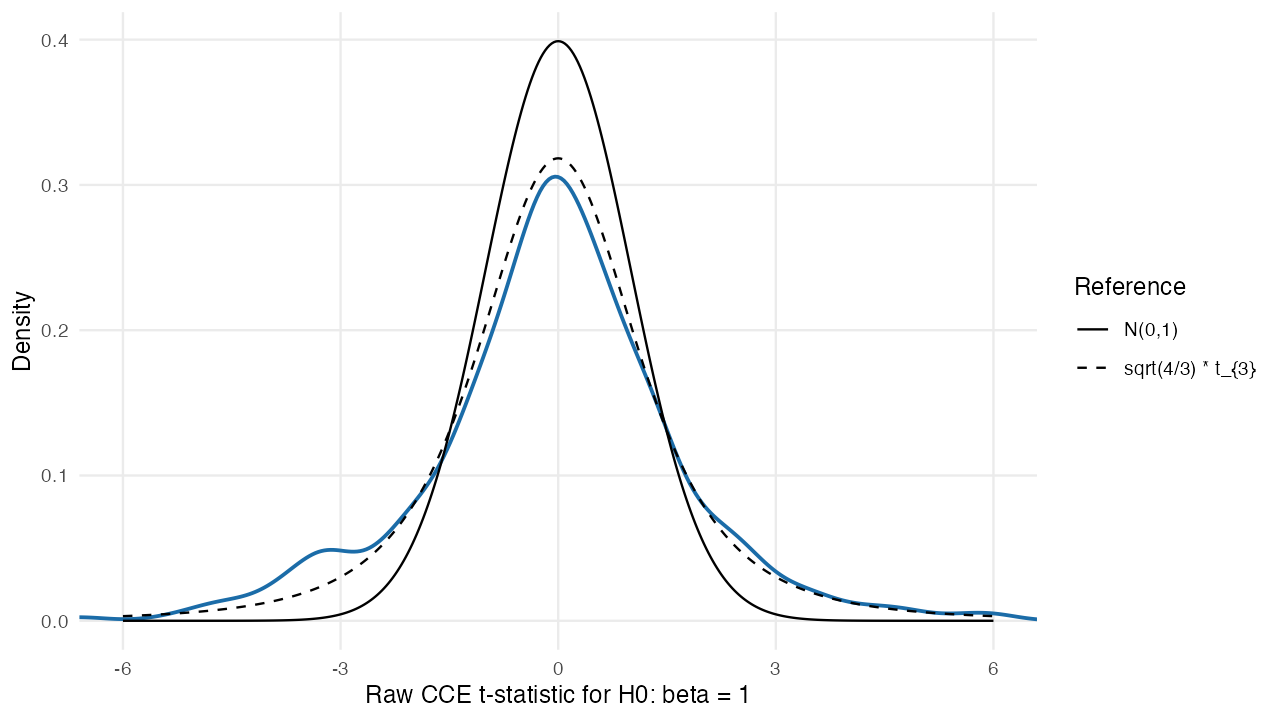
\includegraphics[width=\linewidth]{figA_t_density.png}
\end{minipage}
\hfill
\begin{minipage}{0.48\linewidth}
\centering
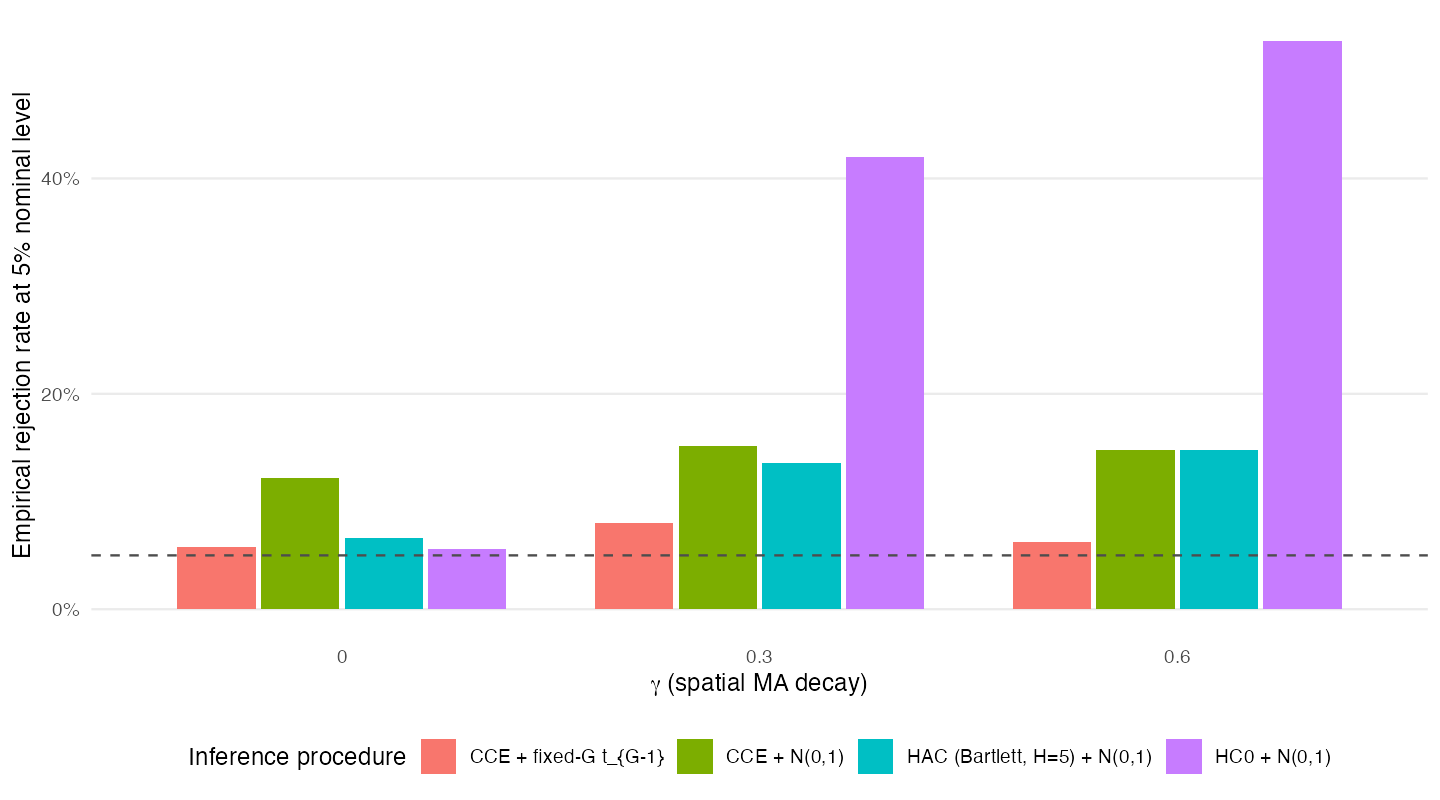
\includegraphics[width=\linewidth]{figB_rejection_rates.png}
\end{minipage}
\caption{Fixed-\(G\) Monte Carlo evidence. Left: raw CCE \(t\)-statistic for \(K=36\), \(\gamma=0.6\), \(G=4\); the BCH reference is wider than \(N(0,1)\). Right: rejection rates for nominal 5 percent tests; the BCH correction is closer to the target size.}
\label{fig:mc-main}
\end{figure}

Figure \ref{fig:mc-main} gives the operational implication. Normal
critical values treat the denominator as precise. BCH use \(t_{G-1}\)
critical values because the variance is estimated from only \(G\) group
scores. This matters in spatial panels. Larger groups can improve
cross-group independence, but they also reduce \(G\). Fixed-\(G\)
inference targets this trade-off.

\begin{figure}[H]
\centering
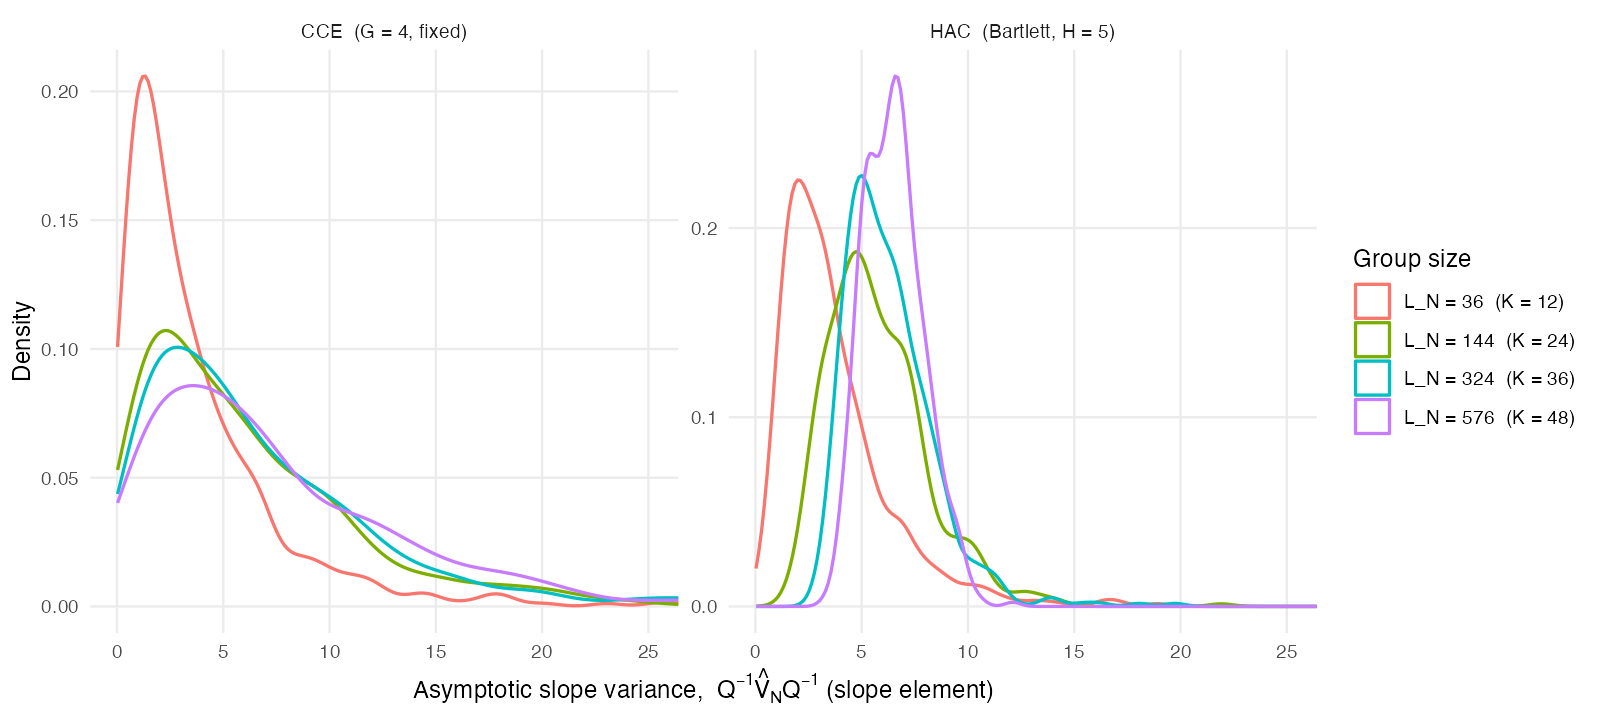
\includegraphics[width=0.62\linewidth]{figC_Vhat_density.png}
\caption{Sampling distribution of the asymptotic-scale variance object. With fixed \(G=4\), the CCE variance estimate remains dispersed as group size grows; the issue is variance-estimator randomness, not only point-estimator convergence.}
\label{fig:mc-vhat}
\end{figure}

Figure \ref{fig:mc-vhat} should not be read as saying that the CCE is
better because its slope-variance distribution is lower. Precision is
valuable only if the covariance estimator is valid for the dependence
structure. The figure is useful for a different reason. It separates two
variance questions. The actual sampling variance of \(\widehat\beta\)
shrinks with \(N\). The plotted object is instead the asymptotic-scale
variance used to studentize \(\sqrt{N}(\widehat\beta-\beta_0)\). Under
fixed \(G\), the CCE estimate of this object remains random because it
is built from only \(G\) group scores. A lower realization of this
object means a smaller standard error in that replication; it does not
by itself mean that the grouping has uncovered more independent
information.

\begin{figure}[H]
\centering
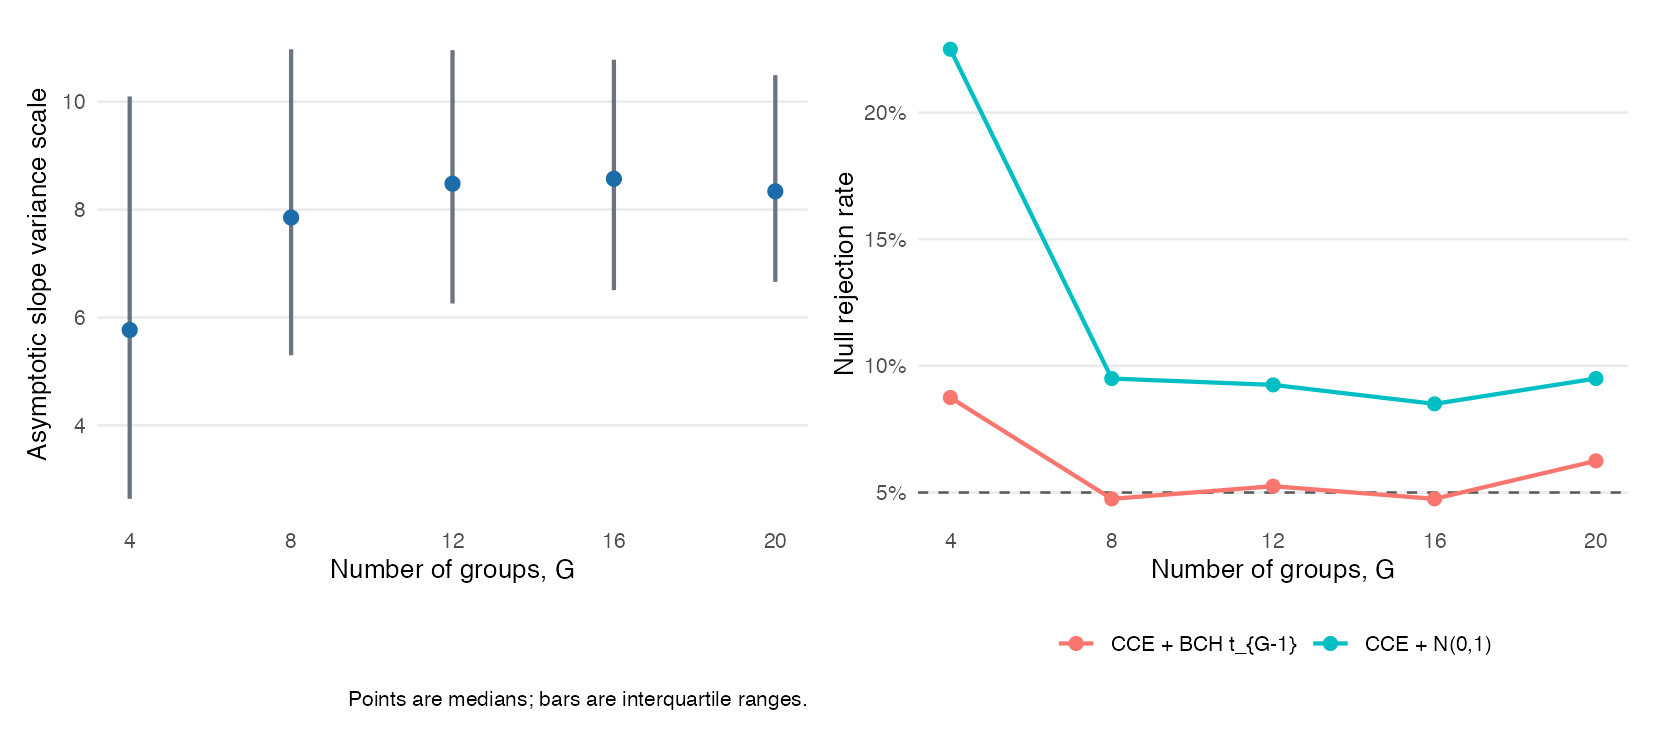
\includegraphics[width=0.92\linewidth]{figD_group_tradeoff.png}
\caption{Monte Carlo trade-off across group counts. The design fixes \(K=60\), \(\gamma=0.6\), and uses balanced contiguous blocks with \(G=4,8,12,16,20\). Left: median and interquartile range of the asymptotic-scale CCE slope variance. Right: empirical rejection rates under the true null.}
\label{fig:mc-g-tradeoff}
\end{figure}

Figure \ref{fig:mc-g-tradeoff} anticipates the empirical application
more directly. Increasing \(G\) gives more degrees of freedom for the
reference distribution, but it also changes the group scores entering
the covariance matrix. The trade-off is therefore not monotone. In this
design, the fixed-\(G\) BCH test is close to nominal size for several
\(G\)'s, while the normal CCE test overrejects, especially when \(G\) is
small. The lesson for the HiClimR application is that \(G\) is not a
tuning parameter for precision. It is a maintained claim about the
spatial scale at which score dependence has been absorbed within groups.
Larger \(G\) can look more precise, but it is credible only if the
resulting groups still leave weak cross-group score dependence.

\section{Empirical Application: Climate and Conflict}

The application follows the data design in \citet{burke2024}. Their
paper studies whether local wealth or national income moderates the
effect of temperature shocks on civil conflict in Africa. It uses a
yearly \(1^\circ\times1^\circ\) grid-cell panel and estimates conflict
models with cell and year fixed effects. For our purpose, the key
feature is the spatially disaggregated weather-conflict panel. It gives
a real setting in which the identifying variation is weather-based but
the appropriate inference units are ambiguous.

We use the monthly weather-conflict layer behind that application. A
cell that is hotter than usual in a given month is closer to a natural
experiment than a comparison of hot and cold places. We therefore use
deviations from each cell's monthly climatology and absorb cell and
year-month fixed effects. This sharpens the inference problem. Climate
deviations may be exogenous, but they are not spatially independent.
Heat anomalies often cover many neighboring cells. Conflict can also
co-move within regions.

\%---------------------------------

\subsection{Why This Application Tests the Grouping Problem}

\%---------------------------------

\citet{burke2024} use African grid cells of roughly
\(1^\circ\times1^\circ\). This scale is useful for identifying local
exposure, but it does not solve inference. Grid-cell clusters are
numerous but implausibly independent. Country clusters are meaningful
but may not match weather systems. Supranational macroregions are closer
to geographers' regional classifications, but still impose boundaries
rather than learning them from climate dynamics. The question is
therefore: what is the relevant spatial unit of climate-conflict
variation?

This setting is informative for group construction for three reasons.
First, temperature anomalies follow a physical process. Their spatial
co-movement can be measured before any conflict regression. Second,
conflict is observed locally, at grid-cell resolution. Third, fixed
effects remove permanent cell differences and common monthly shocks. The
remaining issue is the covariance structure of the regression scores.

HiClimR offers one answer. It groups cells with similar
temperature-anomaly dynamics. It does not group cells with similar
conflict histories. This matters because the grouping rule is tied to
the treatment process, not the outcome. It avoids choosing clusters to
strengthen or weaken the estimated conflict effect.

\begin{table}[H]
\centering
\caption{Why the Burke et al. weather-conflict setting is suitable for BCH group diagnostics}
\label{tab:hbm-grouping}
\begin{tabular}{p{0.26\linewidth}p{0.31\linewidth}p{0.33\linewidth}}
\toprule
Feature of the setting & Econometric advantage & Remaining problem\\
\midrule
Weather deviations from local climatology & Supports a natural-experiment interpretation after fixed effects. & Weather shocks remain spatially correlated.\\
Grid-cell conflict outcomes & Preserves local variation in violence and exposure. & Neighboring cells may not provide independent score information.\\
Multiple possible spatial scales & Allows comparison of coarse and fine dependence groups. & The number of effective groups is not observed directly.\\
Exogenous climate co-movement & Permits pre-outcome construction of climate regions. & Climate homogeneity is not identical to score independence.\\
\bottomrule
\end{tabular}
\end{table}

Our goal is not to replicate the moderation estimates in
\citet{burke2024}. We stress-test the inference layer of the
weather-conflict design. If the association is precise only under fine
groups, the conclusion should be cautious. If it remains precise under
coarse groups, the evidence is stronger.

\%---------------------------------

\subsection{Data}

\%---------------------------------

The empirical database is the derived weather-conflict panel stored with
the project replication files. It was obtained from the replication
package for \citet{burke2024}. The cleaning script crops Berkeley Earth
monthly temperature data to Africa, assigns \(1^\circ\times1^\circ\)
cells to countries using Natural Earth polygons, spatially joins UCDP
GED conflict events to cells, expands events to the months they cover,
and creates monthly conflict counts and indicators. We retain the public
weather-conflict fields and exclude the Atlas wealth and WDI income
variables used for the paper's moderation analysis.

The resulting object is a monthly panel of \(2{,}695\) African grid
cells from 1989 to 2019. Each cell is matched to country identifiers,
coordinates, temperature, monthly climatology, and conflict events. The
main conflict variable is \[
Y_{it}=\mathbf 1\{\text{at least one conflict event occurs in cell } i \text{ during month } t\},
\] equal to one if at least one conflict event occurs in cell \(i\) and
month \(t\). The climate variable is the monthly temperature anomaly \[
A_{it}=temp_{it}-climatology_{im(t)},
\] where \(m(t)\) is calendar month. The BCH application uses
\(1{,}002{,}540\) cell-month observations. Mean conflict incidence is
\(2.916\%\). Mean temperature is \(24.738^\circ C\). Mean anomaly is
\(0.817^\circ C\).

For comparability with the broader project, we also report the
annualized panel. This is not the estimation frequency for the
HiClimR-BCH exercise. It gives a compact summary of scale. A cell-year
is coded as conflicted if any monthly conflict event is observed.

\begin{table}[H]
\centering
\caption{Annual panel coverage and main variables}
\label{tab:descriptive-panel-summary}
\begin{tabular}{lr}
\toprule
Statistic & Value\\
\midrule
Cell-year observations & 83,545\\
Grid cells & 2,695\\
Countries/territories & 51\\
First year & 1989\\
Last year & 2019\\
Annual conflict incidence & 0.103\\
Mean annual temperature & 24.738\\
Mean annual temperature anomaly & 0.817\\
Mean annual conflict events & 0.790\\
\bottomrule
\end{tabular}
\end{table}

\begin{table}[H]
\centering
\caption{Descriptive statistics for the annual grid-cell panel}
\label{tab:descriptive-variable-summary}
\scriptsize
\begin{tabular}{lrrrrrr}
\toprule
Variable & N & Mean & SD & Min & Median & Max\\
\midrule
Conflict events & 83,545 & 0.790 & 7.559 & 0.000 & 0.000 & 1,365.000\\
Conflict indicator & 83,545 & 0.103 & 0.304 & 0.000 & 0.000 & 1.000\\
Conflict months & 83,545 & 0.350 & 1.478 & 0.000 & 0.000 & 12.000\\
Temperature & 83,545 & 24.738 & 3.433 & 11.089 & 25.033 & 31.763\\
Temperature anomaly & 83,545 & 0.817 & 0.430 & -0.965 & 0.835 & 2.810\\
Climatology & 83,545 & 23.921 & 3.409 & 11.108 & 24.255 & 29.972\\
\bottomrule
\end{tabular}
\end{table}

The tables establish scale, but not the time structure of identifying
variation. Figure \ref{fig:time-descriptives} therefore compares annual
aggregation with the monthly variation used in the BCH application.

\begin{figure}[H]
\centering
\begin{minipage}{0.49\linewidth}
\centering
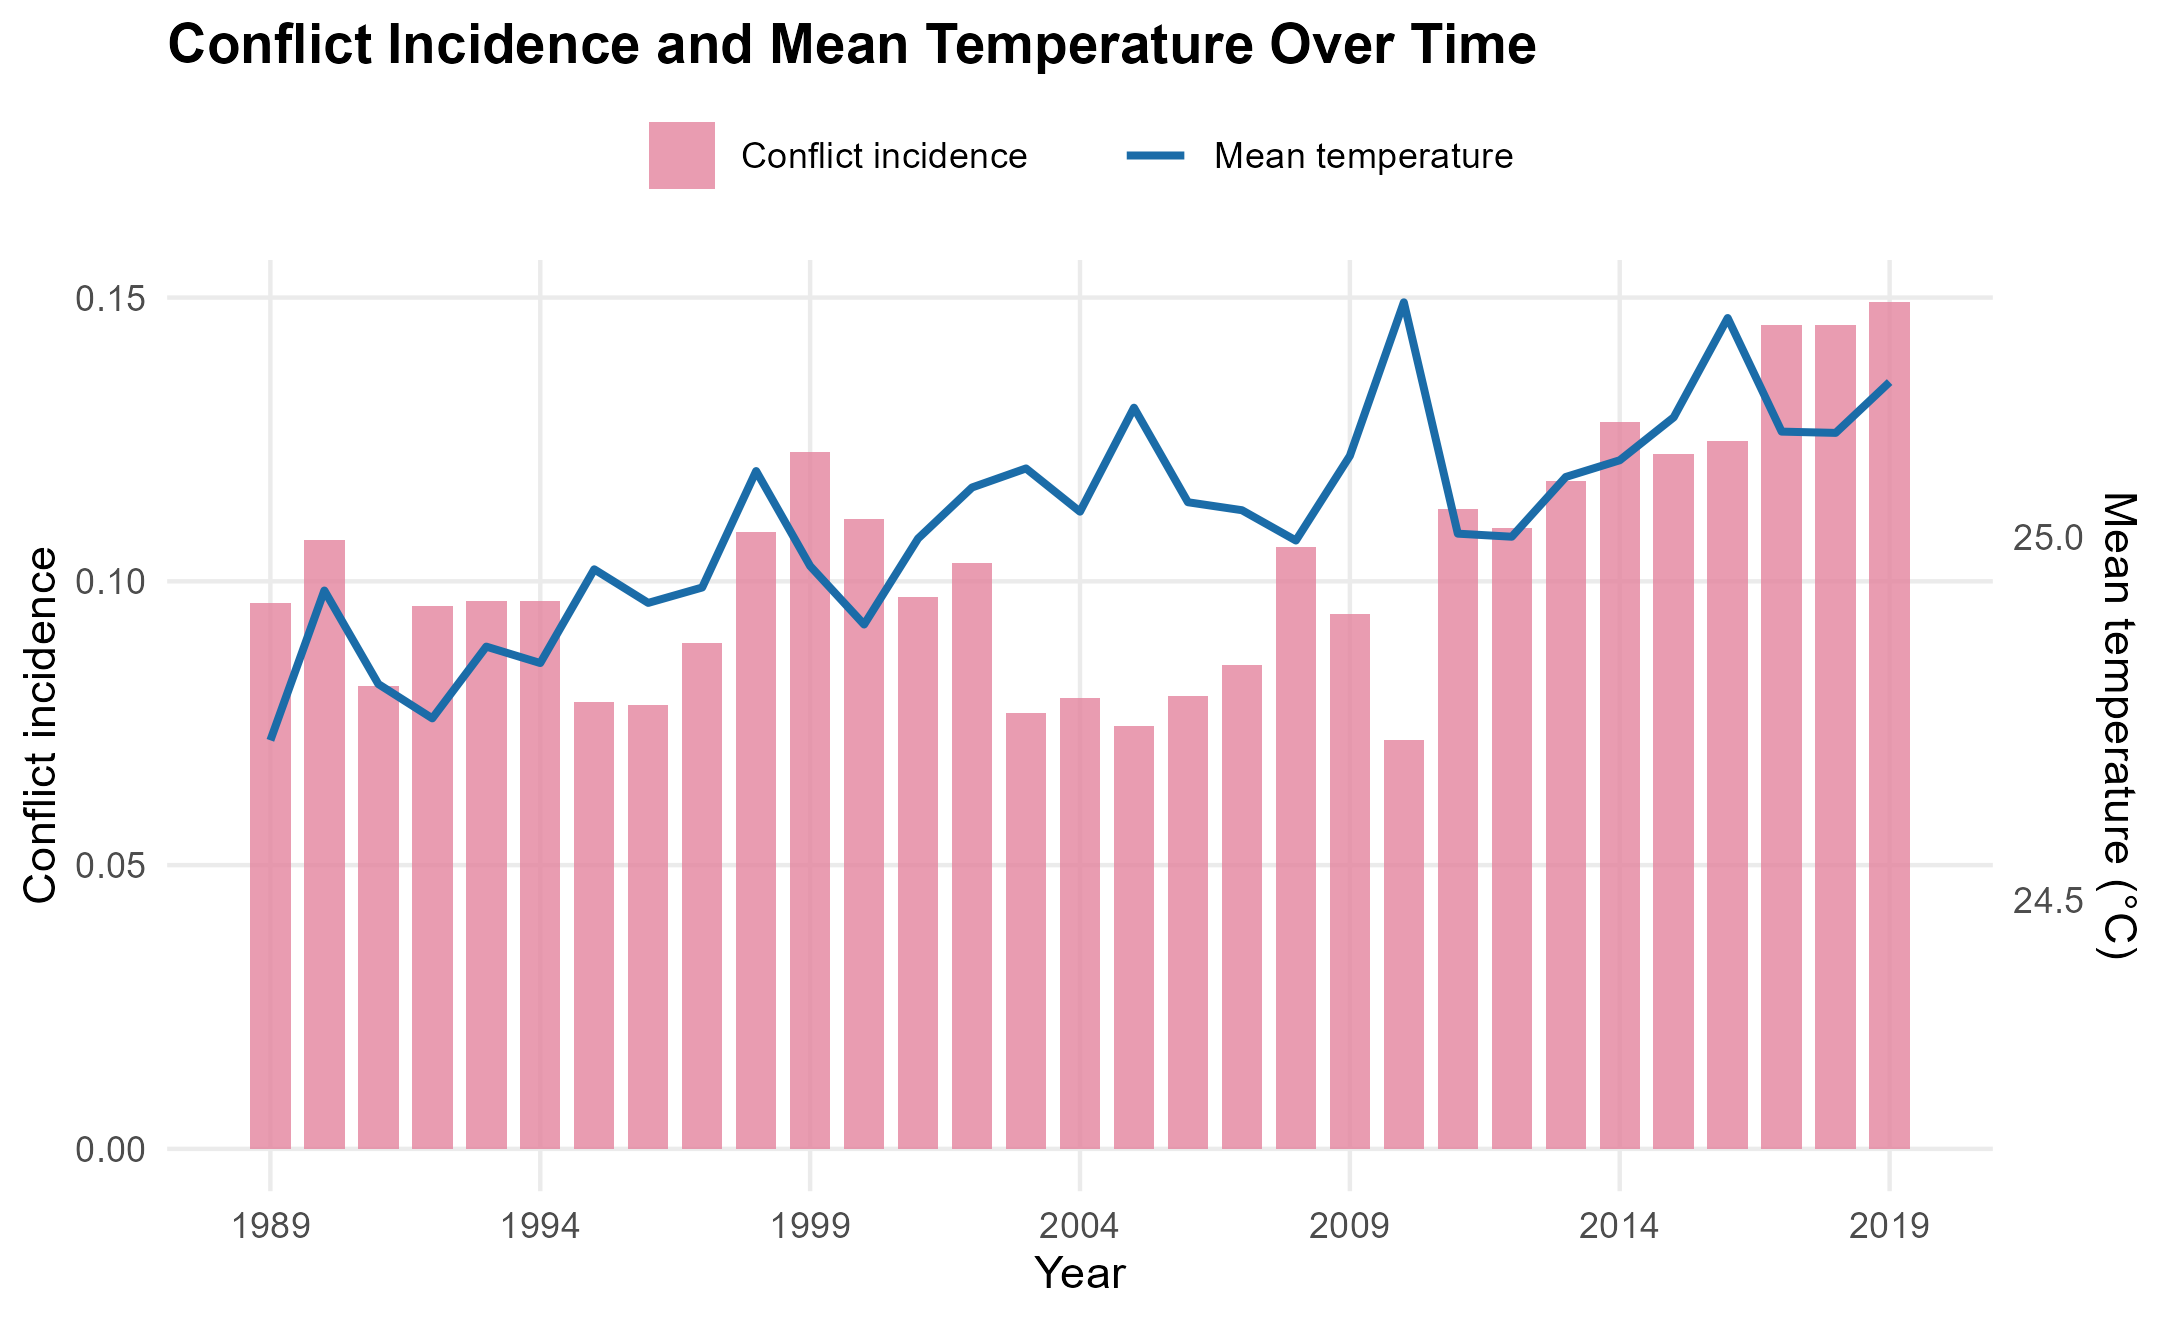
\includegraphics[width=\linewidth]{annual_conflict_temperature.png}
\end{minipage}
\hfill
\begin{minipage}{0.49\linewidth}
\centering
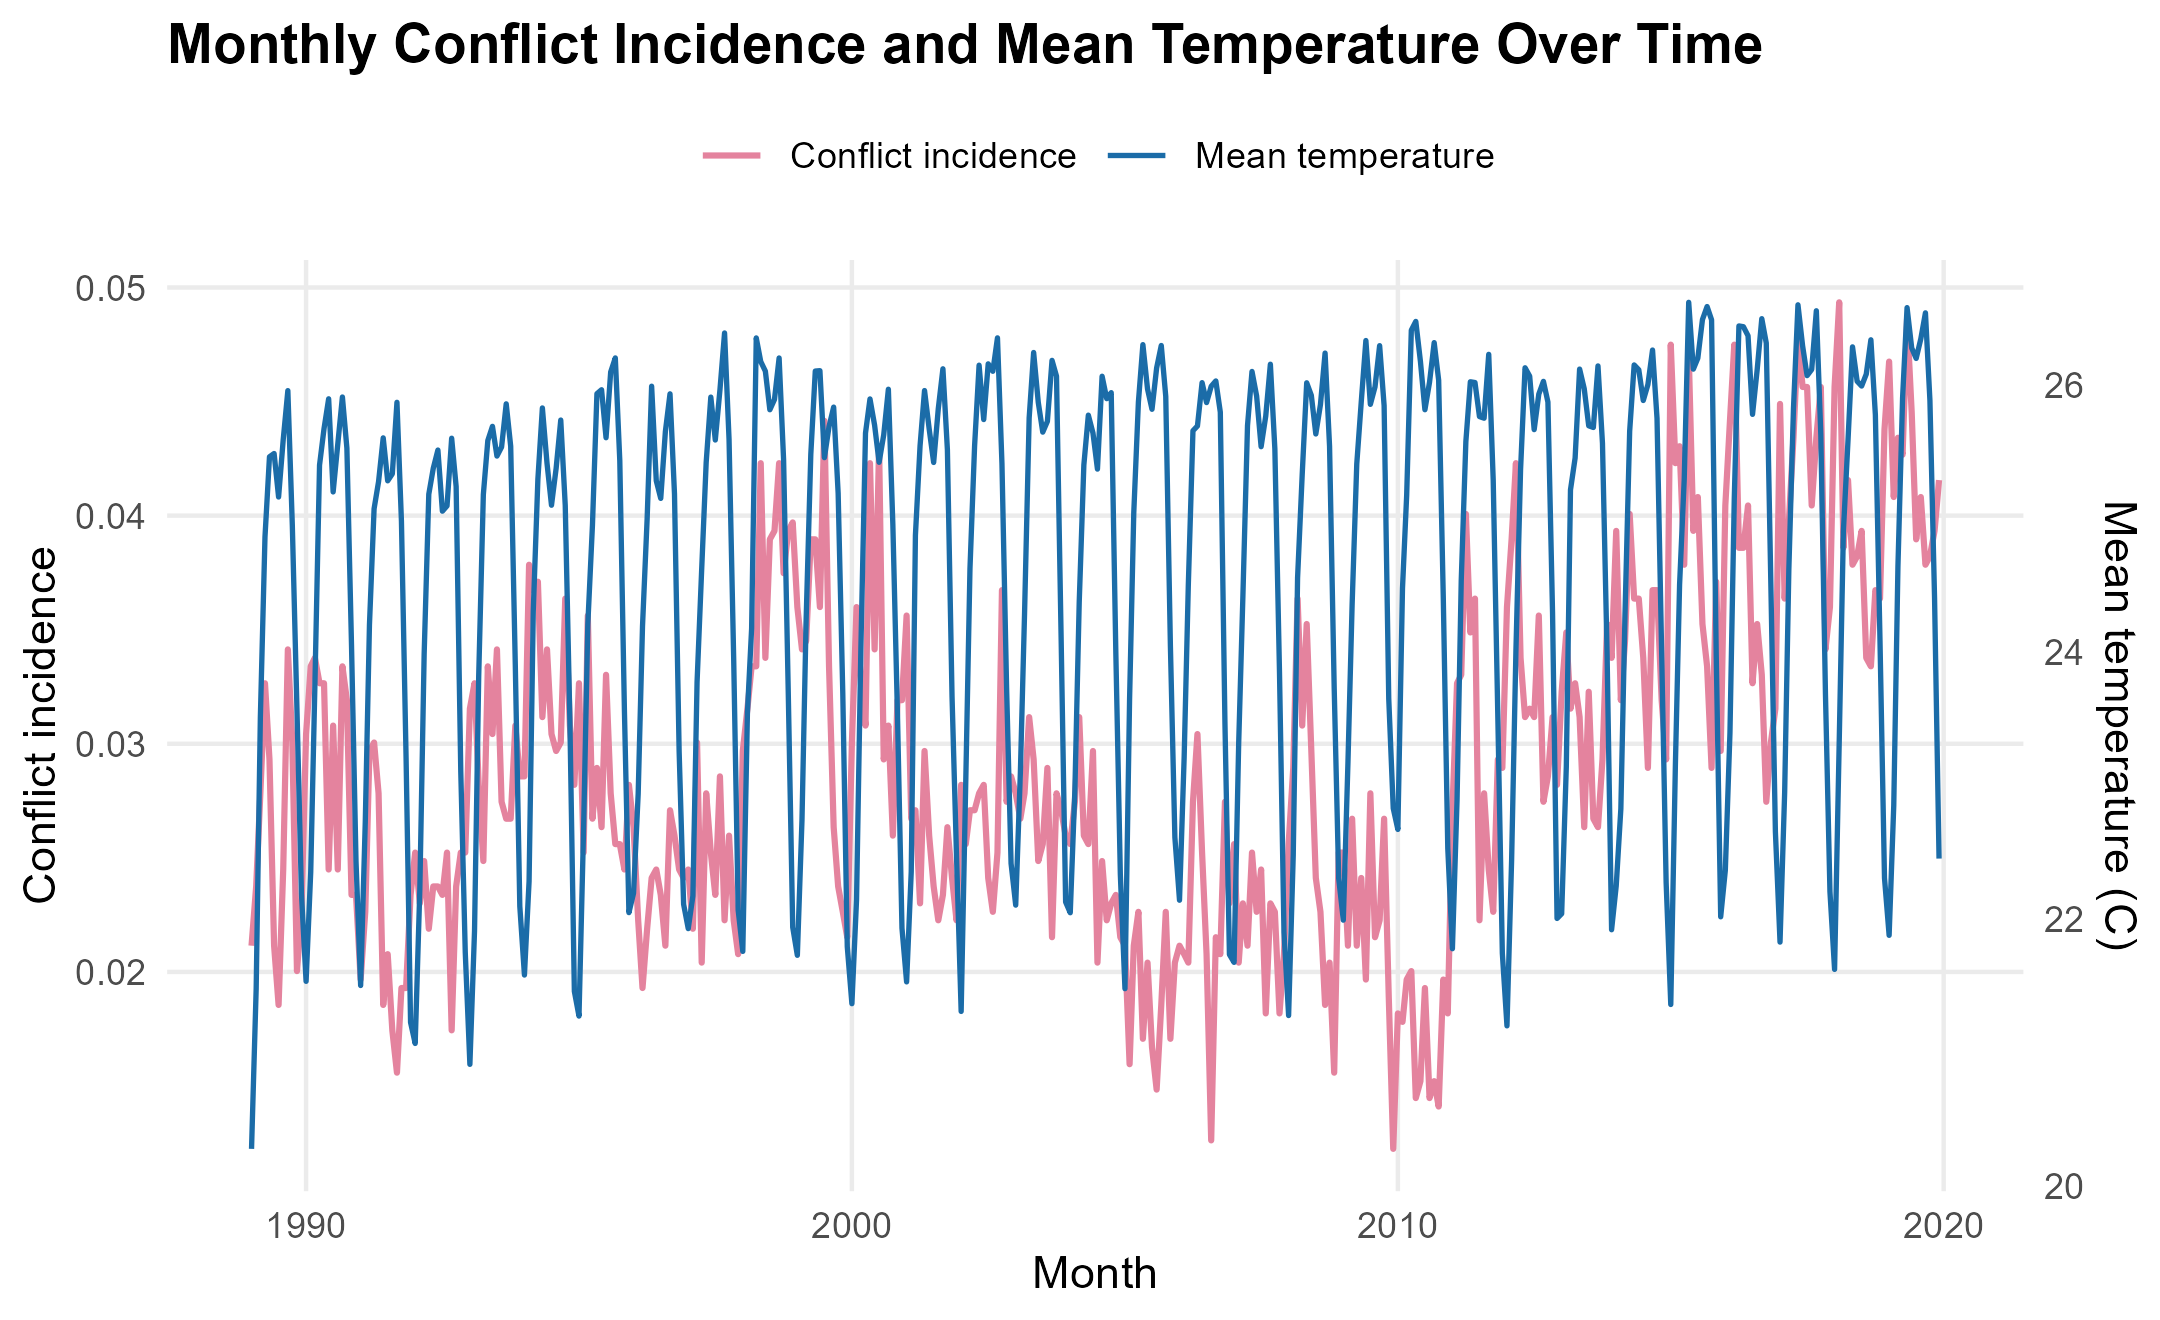
\includegraphics[width=\linewidth]{monthly_conflict_temperature.png}
\end{minipage}
\caption{Time-series descriptives from the project copy. The annual view shows slow co-movement; the monthly view preserves the short-run variation used in the BCH application.}
\label{fig:time-descriptives}
\end{figure}

Figure \ref{fig:time-descriptives} motivates the monthly design. Annual
data show broad co-movement but compress the shocks that identify
\(\beta\). Monthly data preserve short-run anomalies and provide many
observations within each candidate group. The remaining question is
spatial: are those observations independent enough across cells? Figure
\ref{fig:spatial-descriptives} maps the relevant spatial structure.

\begin{figure}[H]
\centering
\begin{minipage}{0.32\linewidth}
\centering
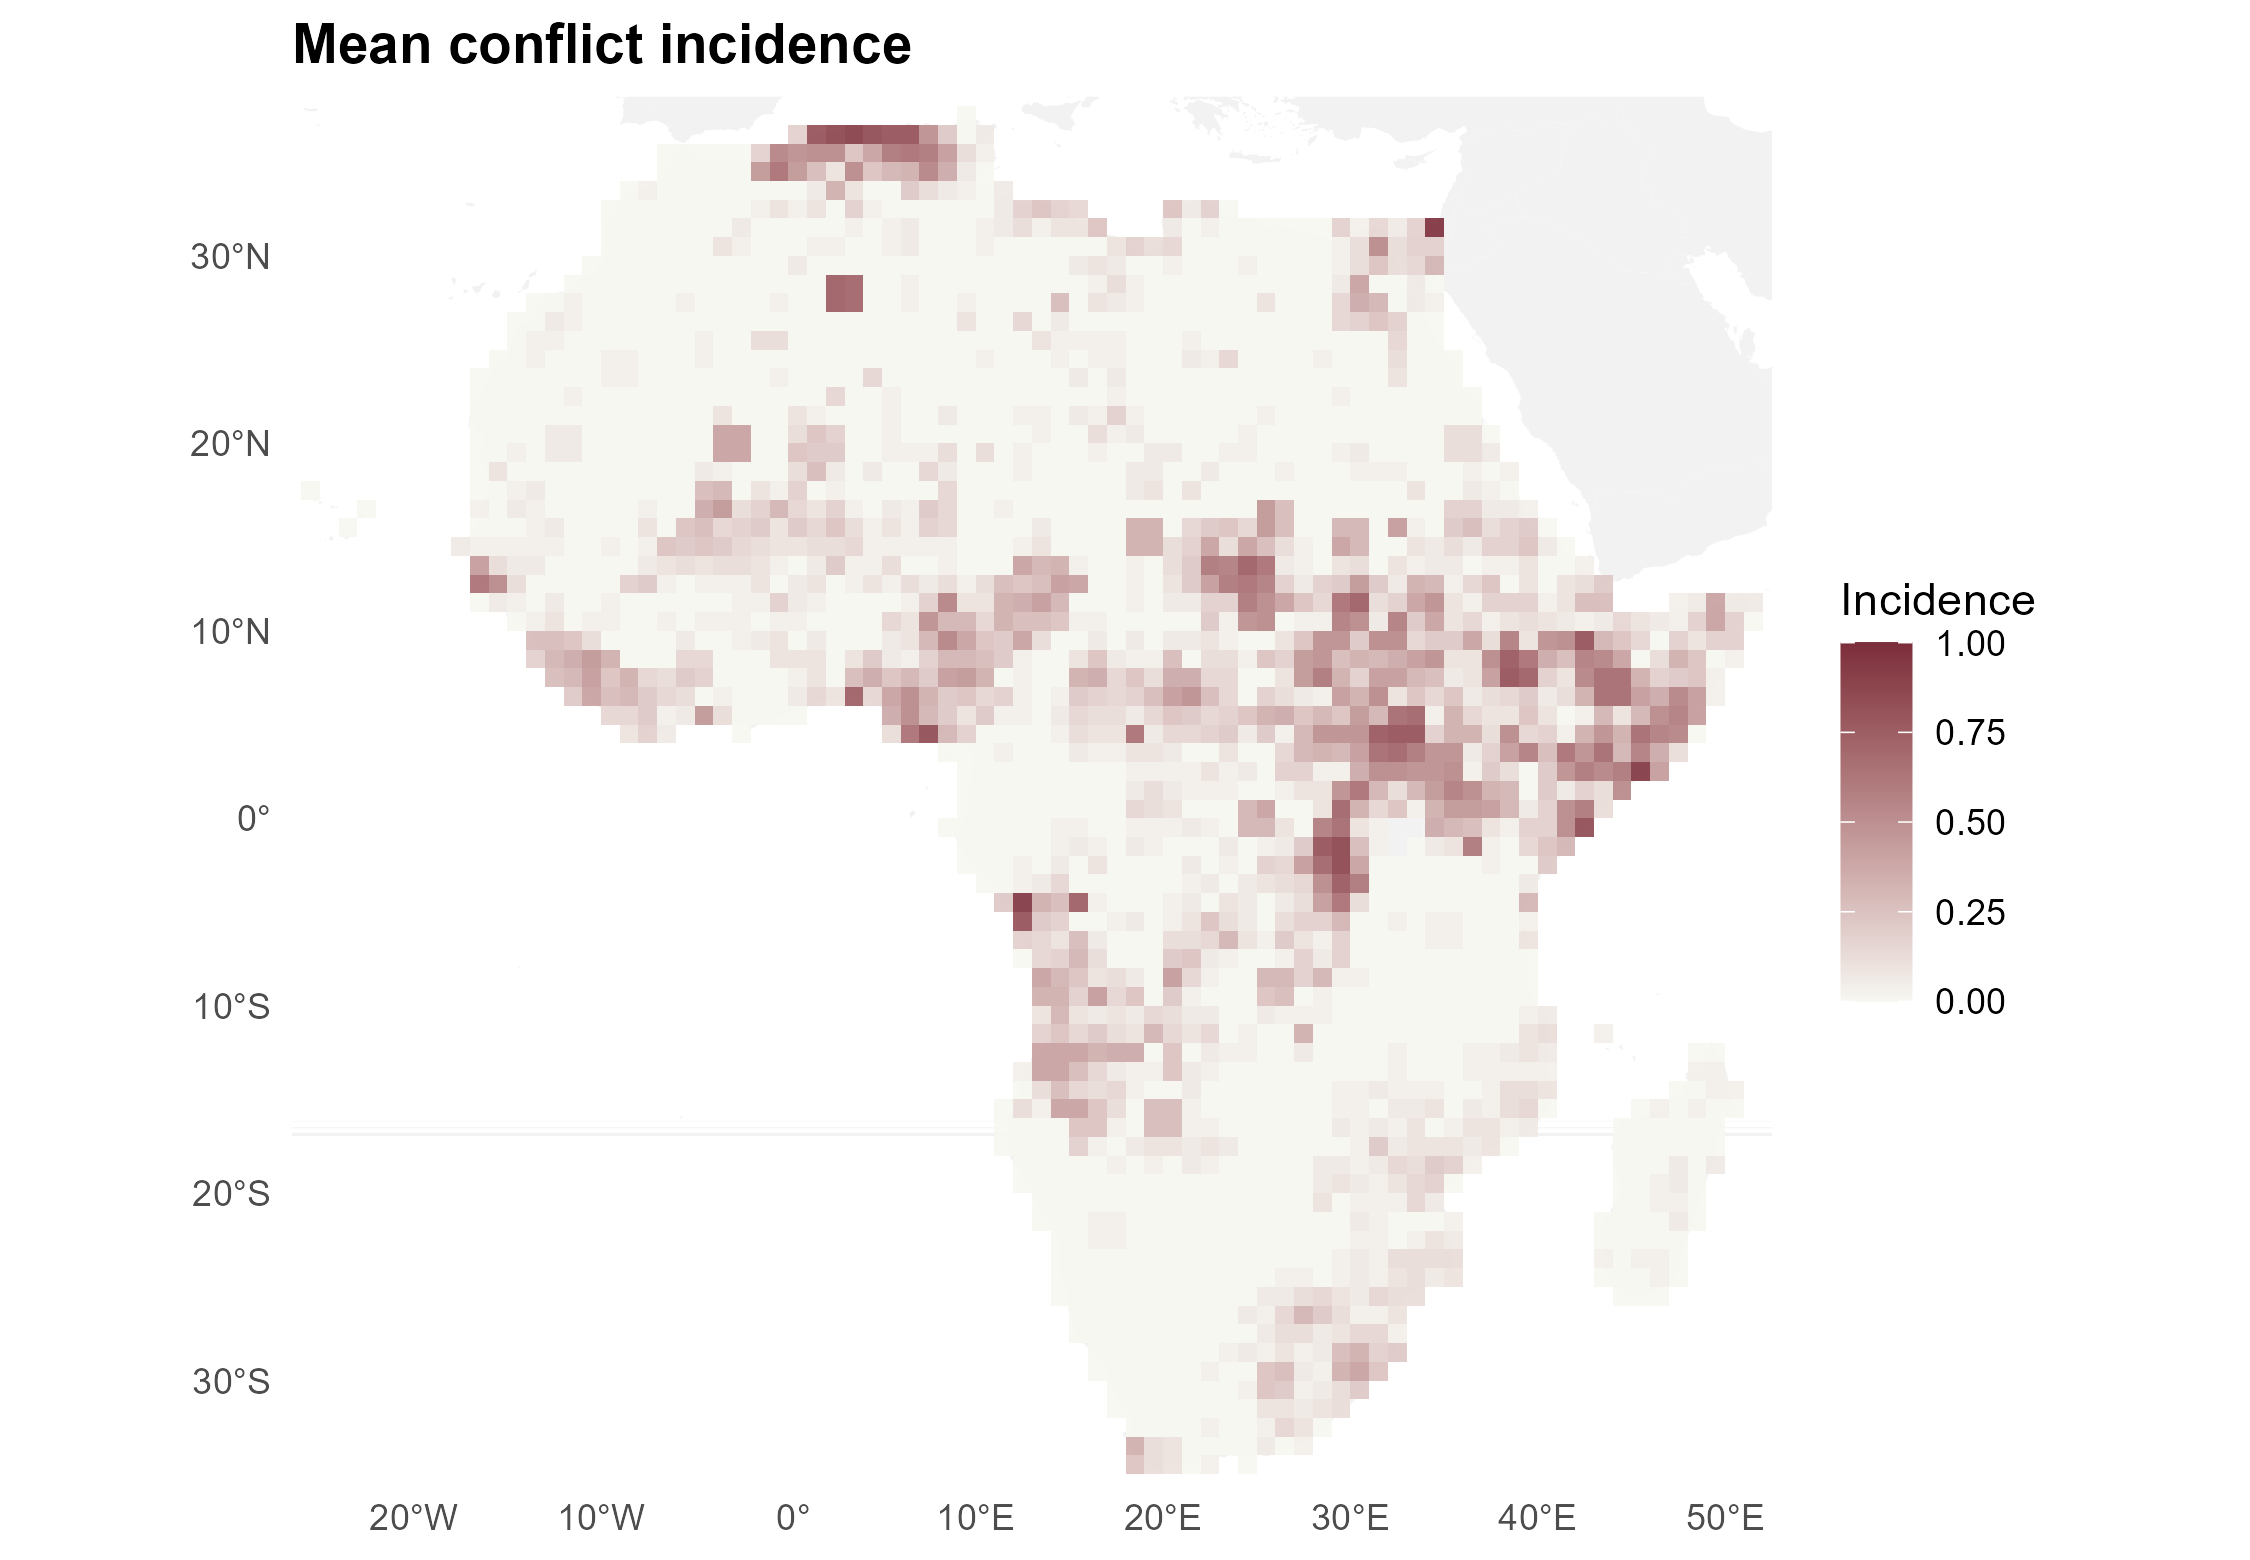
\includegraphics[width=\linewidth]{map_conflict_incidence.png}
\vspace{0.2em}
{\scriptsize (a) Conflict incidence}
\end{minipage}
\hfill
\begin{minipage}{0.32\linewidth}
\centering
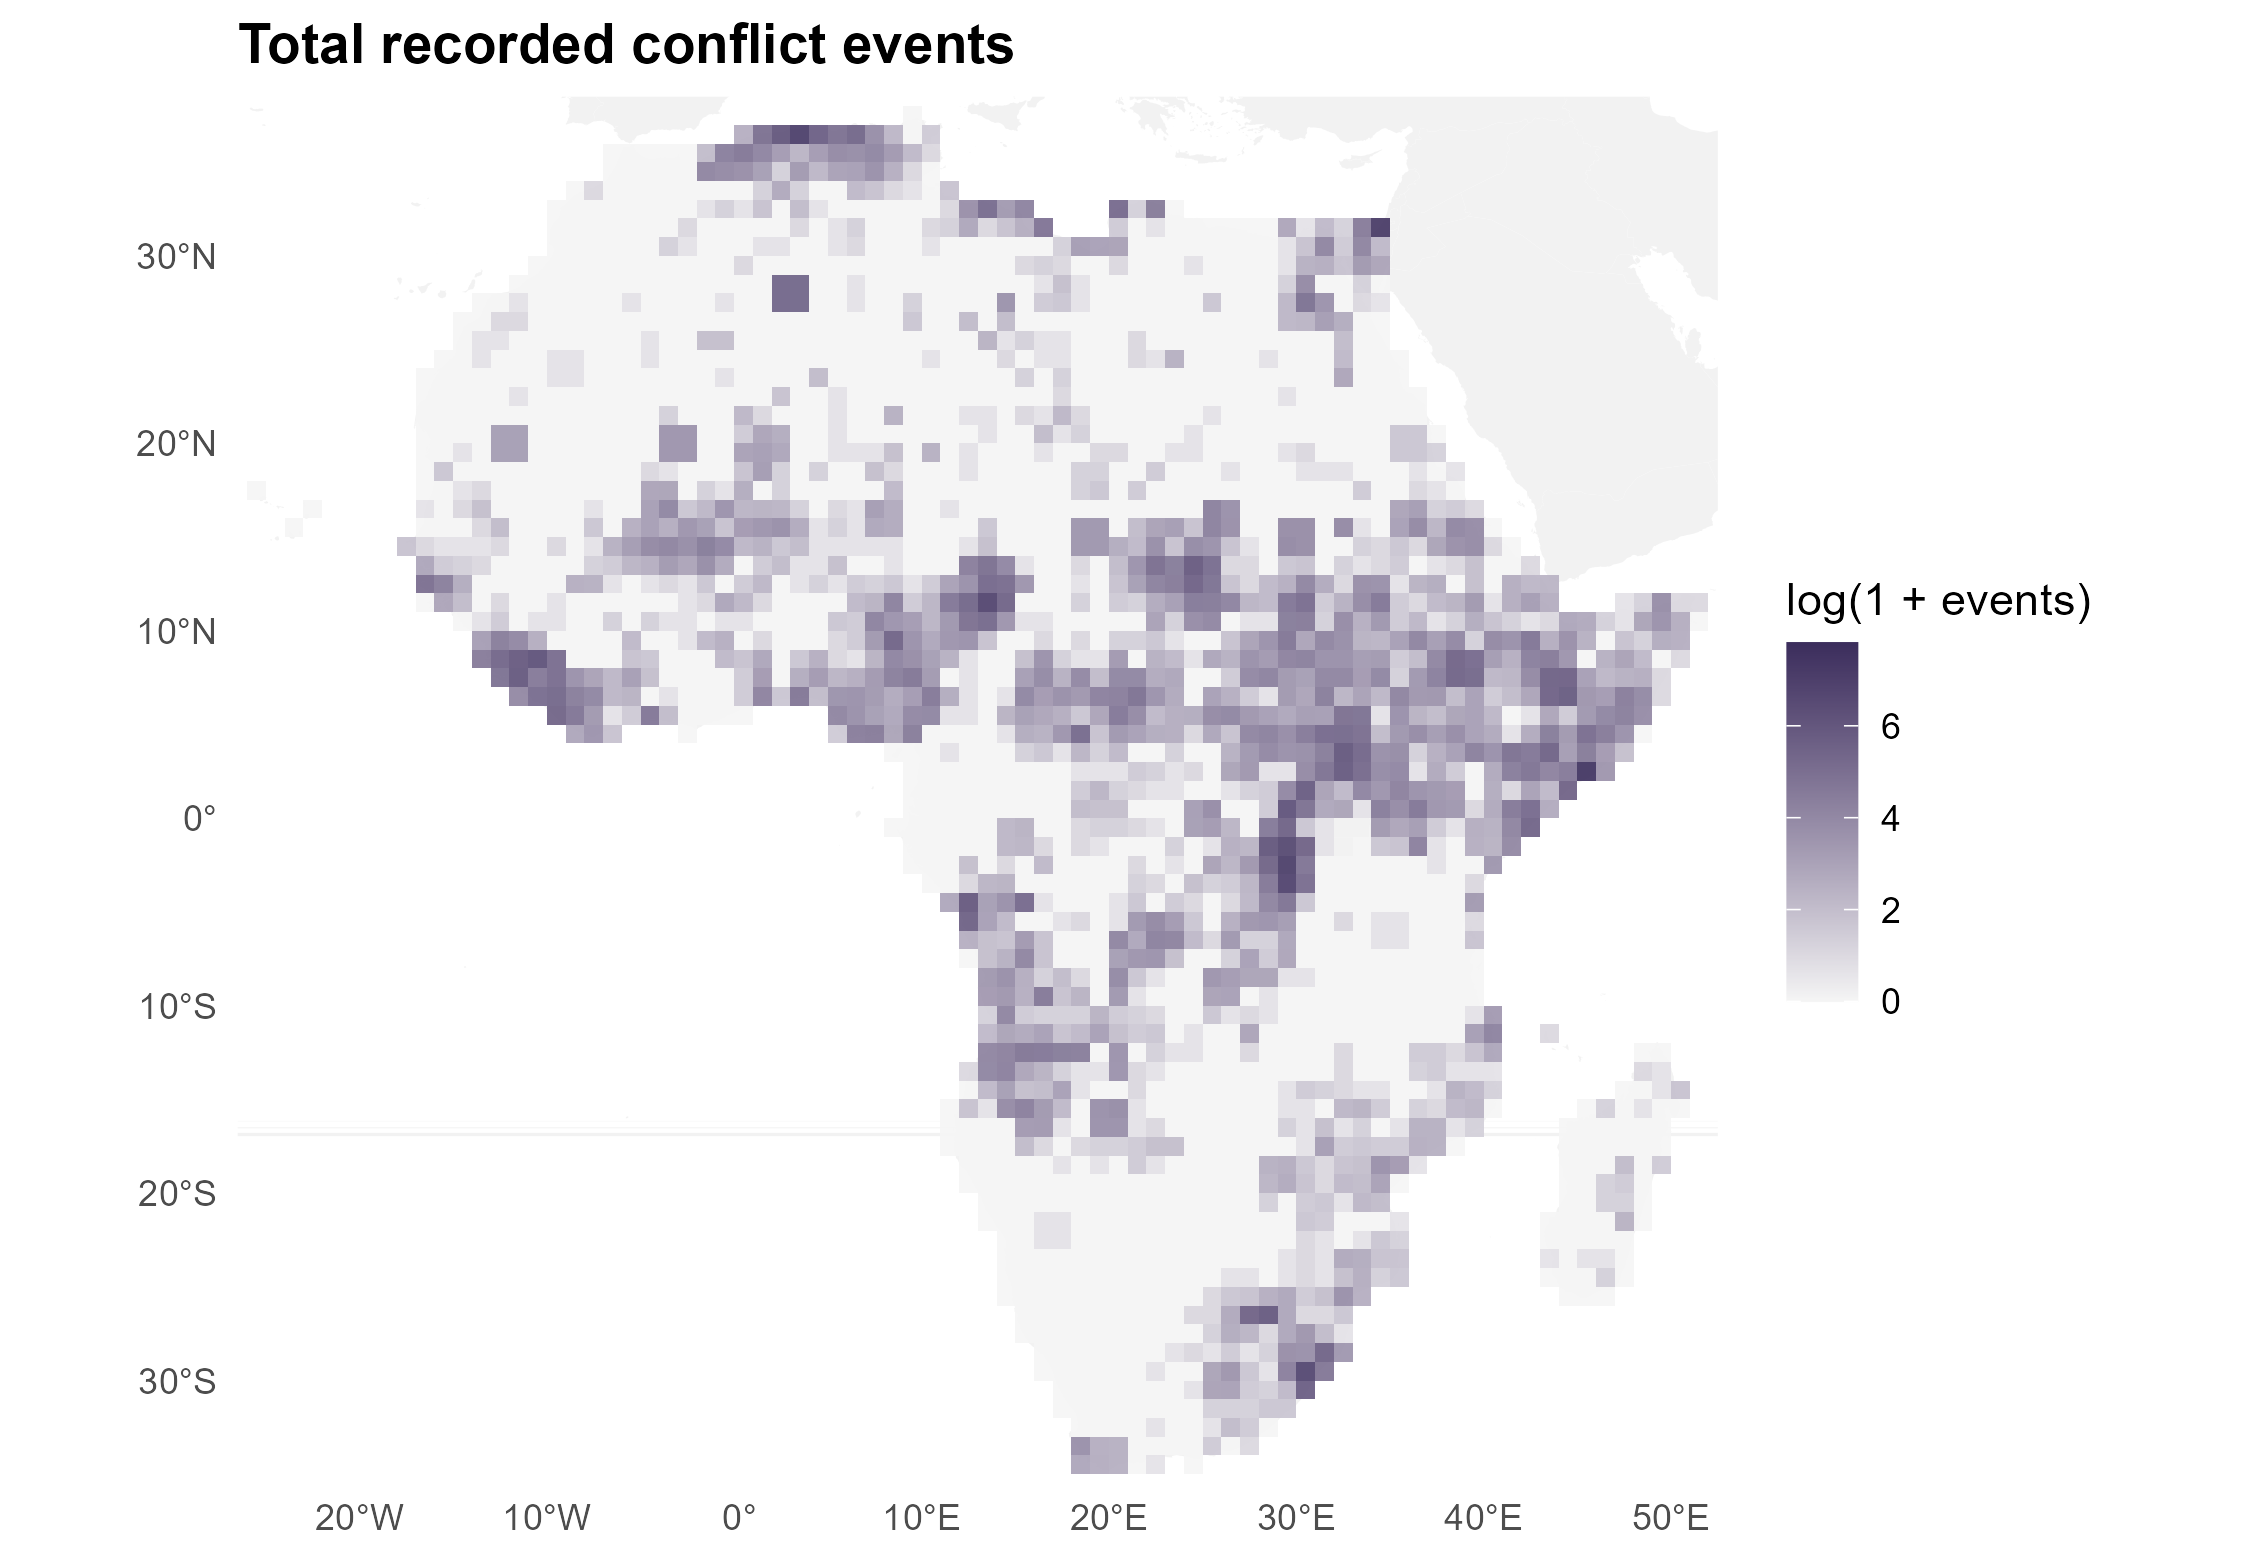
\includegraphics[width=\linewidth]{map_conflict_events.png}
\vspace{0.2em}
{\scriptsize (b) Conflict events}
\end{minipage}
\hfill
\begin{minipage}{0.32\linewidth}
\centering
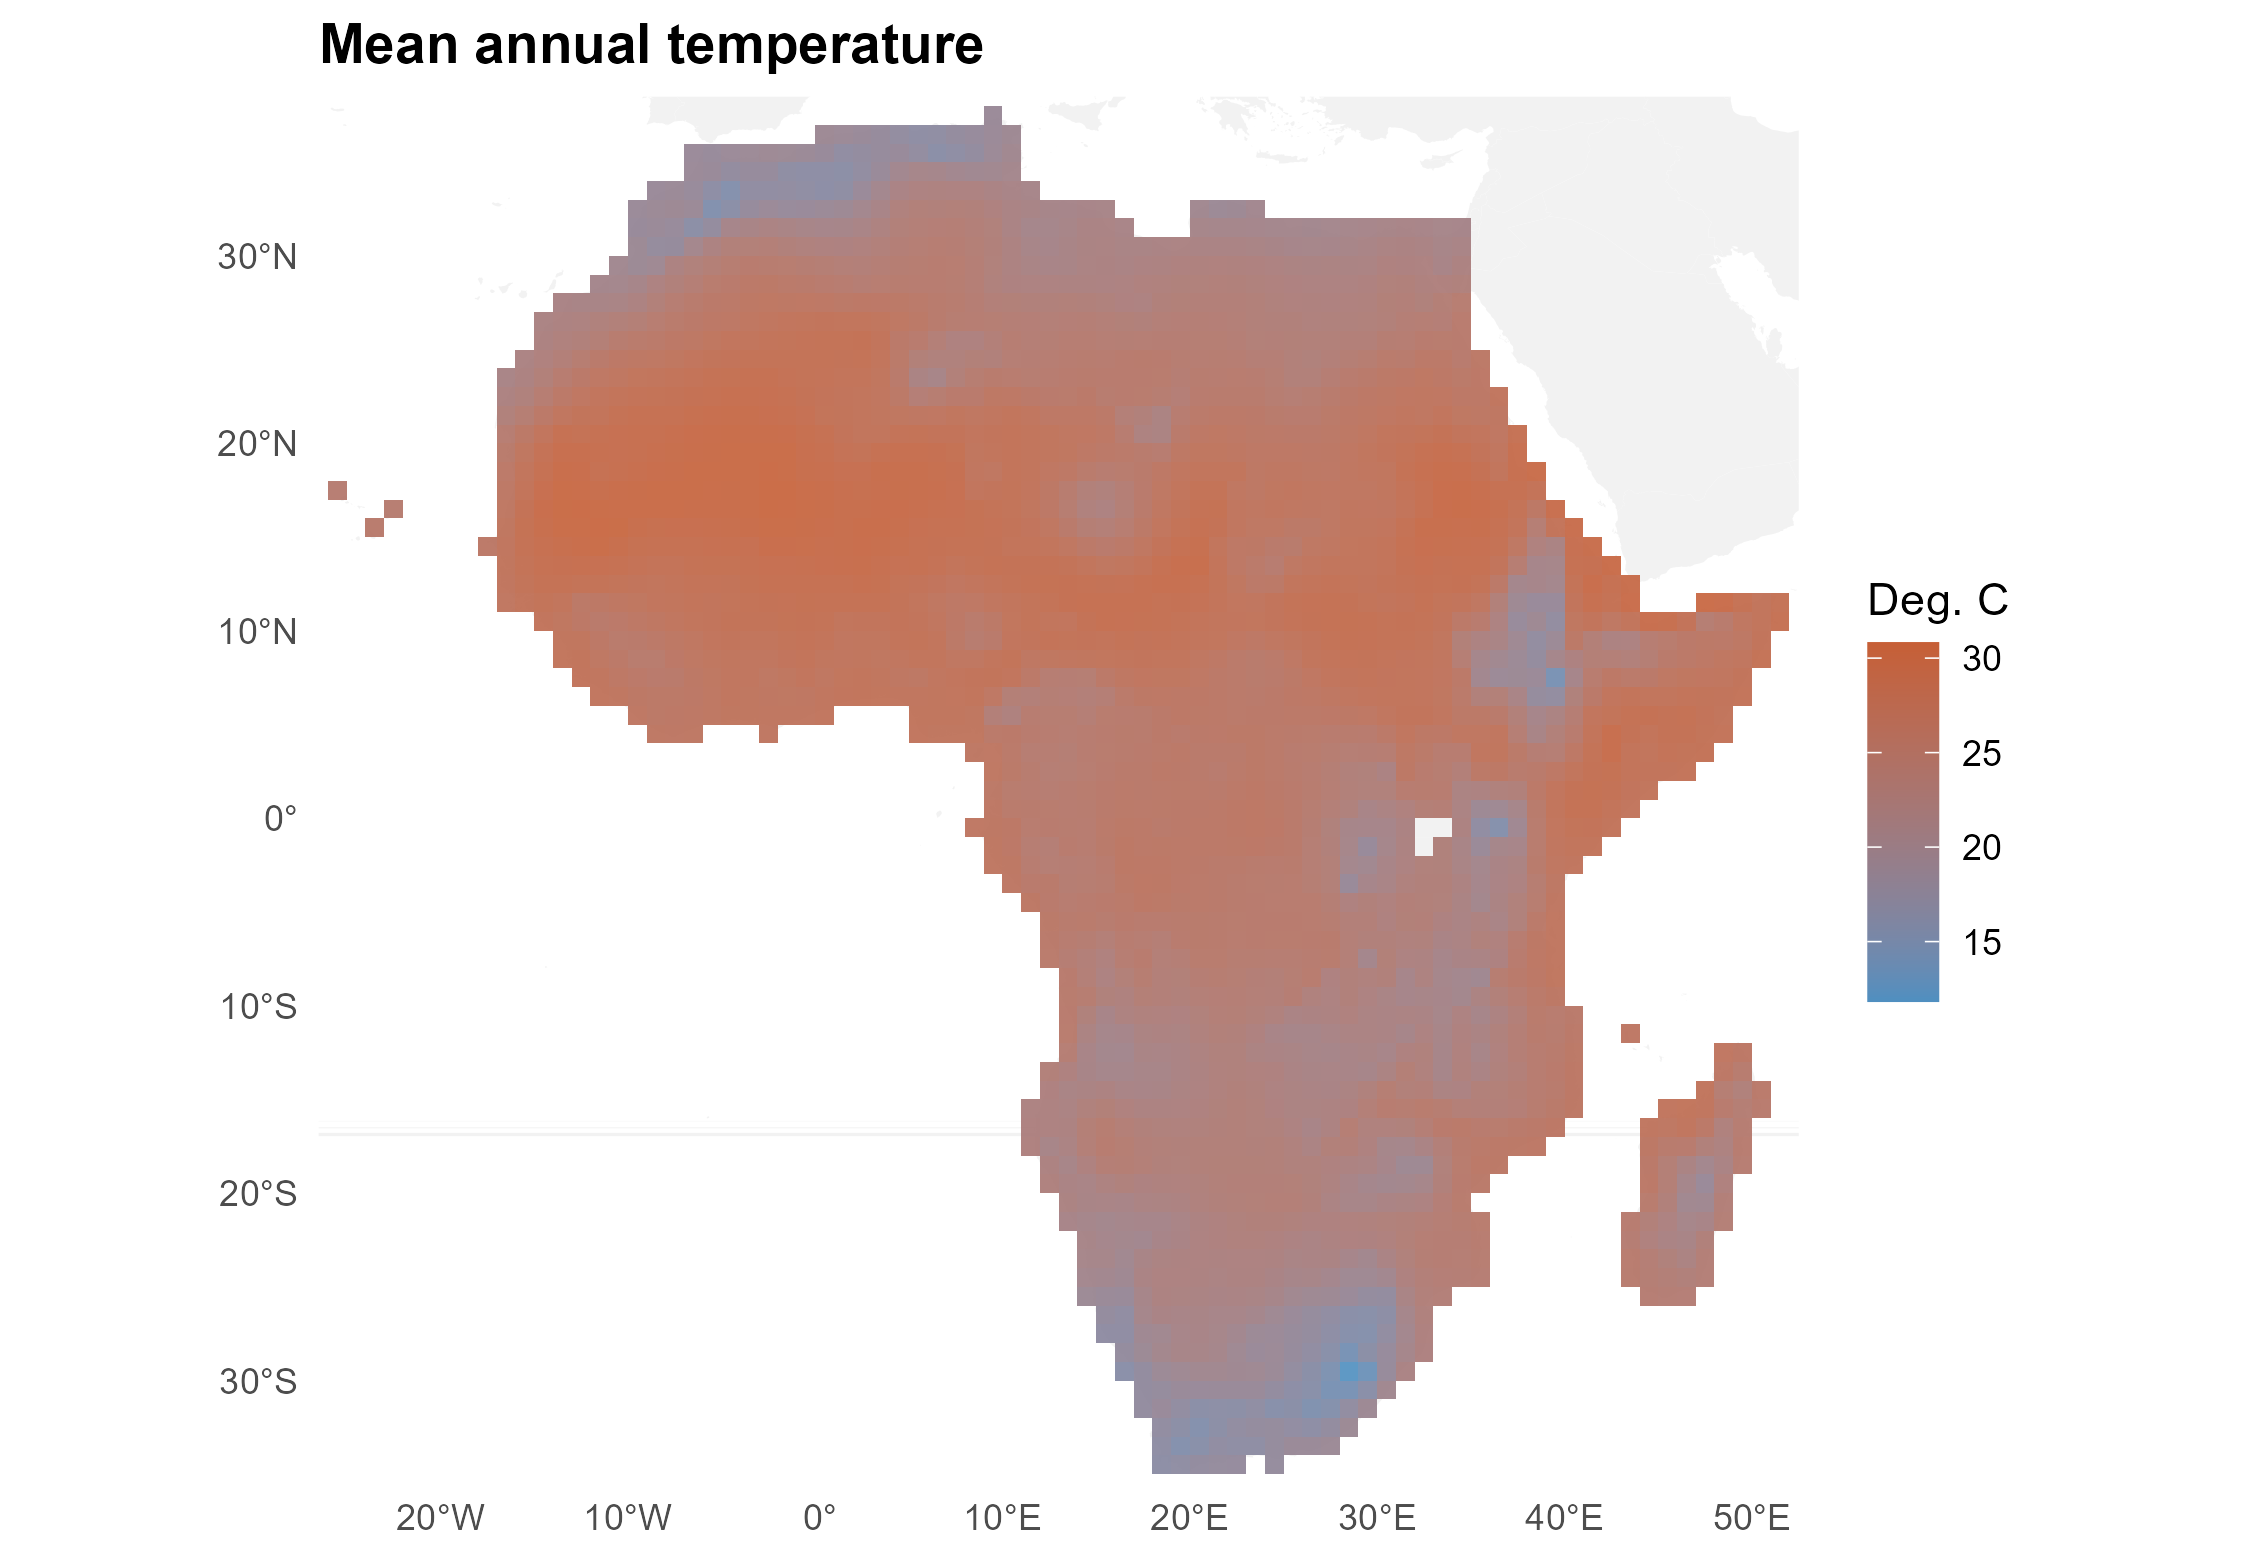
\includegraphics[width=\linewidth]{map_mean_temperature.png}
\vspace{0.2em}
{\scriptsize (c) Mean temperature}
\end{minipage}
\caption{Spatial descriptives for the African grid-cell panel. Conflict and temperature both have visible spatial structure. This motivates spatial inference rather than treating cell-months as independent.}
\label{fig:spatial-descriptives}
\end{figure}

Figure \ref{fig:spatial-descriptives} shows that neither conflict nor
temperature is spatially featureless. This is not evidence that hot
places mechanically have more conflict; cell fixed effects remove
permanent level differences. The figure matters because nearby cells may
share weather systems and unobserved shocks. The monthly panel is
therefore useful for BCH, but only with a defensible spatial grouping
rule.

\%---------------------------------

\subsection{Empirical Specification}

\%---------------------------------

The baseline linear probability model is \begin{equation}
Y_{it}=\beta A_{it}+\alpha_i+\delta_t+\varepsilon_{it},
\label{eq:empirical}
\end{equation} where \(\alpha_i\) are grid-cell fixed effects and
\(\delta_t\) are year-month fixed effects. The coefficient is identified
by within-cell deviations from normal monthly temperature, compared
across cells in the same month. The design removes permanent cell
differences and aggregate monthly shocks. The coefficient is causal only
if residual temperature anomalies are as-good-as random conditional on
these fixed effects.

For OLS, the relevant BCH group contribution is the score \[
S_g(\widehat\beta)=X_g'\widehat e_g,
\] not the outcome alone and not temperature alone. Clustering on
temperature is therefore not a substitute for BCH assumptions. It is a
way to define large, physically interpretable groups before computing
clustered inference.

The broader project establishes the sign and scale of the
weather-conflict association. This section asks a narrower question.
Does the conclusion survive when independent information is a small
number of climate regions rather than thousands of cells?

\%---------------------------------

\subsection{HiClimR Climate Groups}

\%---------------------------------

HiClimR is a hierarchical climate regionalization algorithm. We form a
\(2{,}695\times372\) matrix. Rows are cells; columns are months. Entry
\((i,t)\) is \(A_{it}\). HiClimR detrends and standardizes each row,
computes correlation distances, and builds a clustering tree. Cutting
the tree at \(G=k\) gives \(G\) climate groups.

This addresses the grouping problem directly. Administrative borders are
convenient but not physically privileged. Country groups can be too
coarse for local violence and too political for weather shocks.
Grid-cell clustering is usually too fine for spatial dependence. HiClimR
is an intermediate choice: regions follow climate co-movement at the
outcome's spatial resolution, without using conflict outcomes.

After the data section shows spatial structure, Figure
\ref{fig:hiclmr-map} starts with the coarsest climate grouping. It asks
whether the panel can be summarized by a few large regions, as
fixed-\(G\) inference requires.

\begin{figure}[H]
\centering
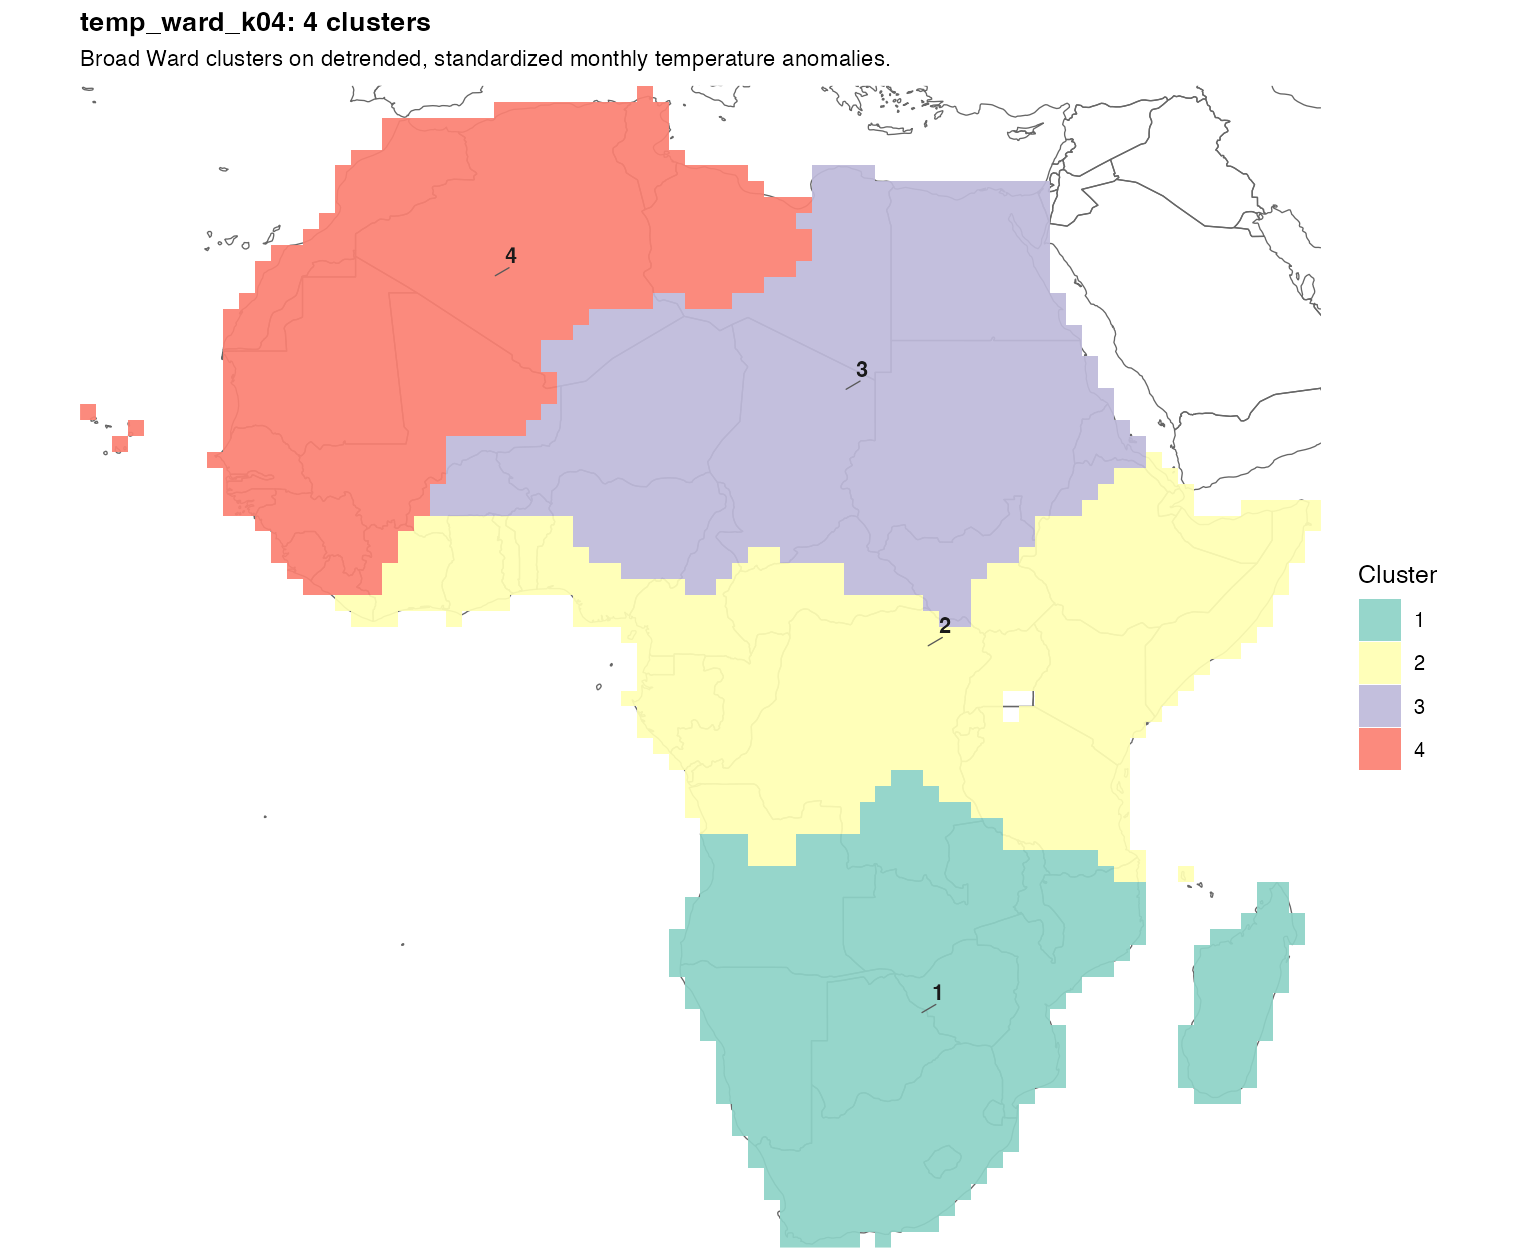
\includegraphics[width=0.72\linewidth]{temp_ward_k04.png}
\caption{Preferred coarse HiClimR partition. The \(G=4\) Ward partition gives large, nearly contiguous climate groups, which is closest to the BCH requirement of a fixed small number of large groups.}
\label{fig:hiclmr-map}
\end{figure}

Figure \ref{fig:hiclmr-map} is a benchmark, not proof that \(G=4\) is
correct. It shows that climate groups can be large, spatially coherent,
and chosen before observing conflict outcomes. This makes the later
\(G=4\) inference conservative; finer partitions must be justified by
diagnostics, not only by smaller standard errors.

Table \ref{tab:cluster-diagnostics} reports the candidate partitions.
The \(G=4\) partition is most defensible for BCH because all groups are
large. The smallest contains 618 cells. Finer partitions raise
within-cluster temperature homogeneity, but some groups become small and
unbalanced. In fixed-\(G\) inference, larger \(G\) is not automatically
better.

\begin{table}[H]
\centering
\caption{HiClimR partitions used as candidate BCH groups}
\label{tab:cluster-diagnostics}
\begin{tabular}{lrrrrr}
\toprule
Proposal & \(G\) & Cell size min/med/max & Intra corr. & Inter corr. & Method\\
\midrule
Broad Ward climate partition & 4 & 618/670/738 & 0.683 & 0.239 & Ward\\
Regional-linkage climate partition & 8 & 66/369/636 & 0.763 & 0.213 & Regional\\
Contiguity-weighted Ward partition & 12 & 66/196/396 & 0.816 & 0.210 & Ward + contig.\\
PCA-filtered Ward partition & 16 & 90/168/279 & 0.849 & 0.229 & Ward + PCA\\
Hybrid Ward-regional partition & 20 & 14/124/472 & 0.855 & 0.209 & Hybrid\\
\bottomrule
\end{tabular}
\end{table}

Table \ref{tab:cluster-diagnostics} reports intra- and inter-cluster
temperature-anomaly correlations. Higher intra-cluster correlation means
more similar anomaly dynamics within groups. Lower inter-cluster
correlation means group mean anomaly series are more separated. These
are climate diagnostics, not proof of BCH validity. BCH validity
concerns the score process. Residual or score diagnostics remain
necessary.

The comparison across \(G\) is also inferential. \(G=4\) treats Africa
as a few large climate regions. \(G=8\) and \(G=12\) keep moderate group
sizes. \(G=16\) and \(G=20\) are closer to descriptive regionalization:
they improve climate homogeneity but create small groups.

Figure \ref{fig:all-clusters} visualizes the trade-off in Table
\ref{tab:cluster-diagnostics}: numerical climate homogeneity must still
correspond to geographically interpretable groups.

\begin{figure}[H]
\centering
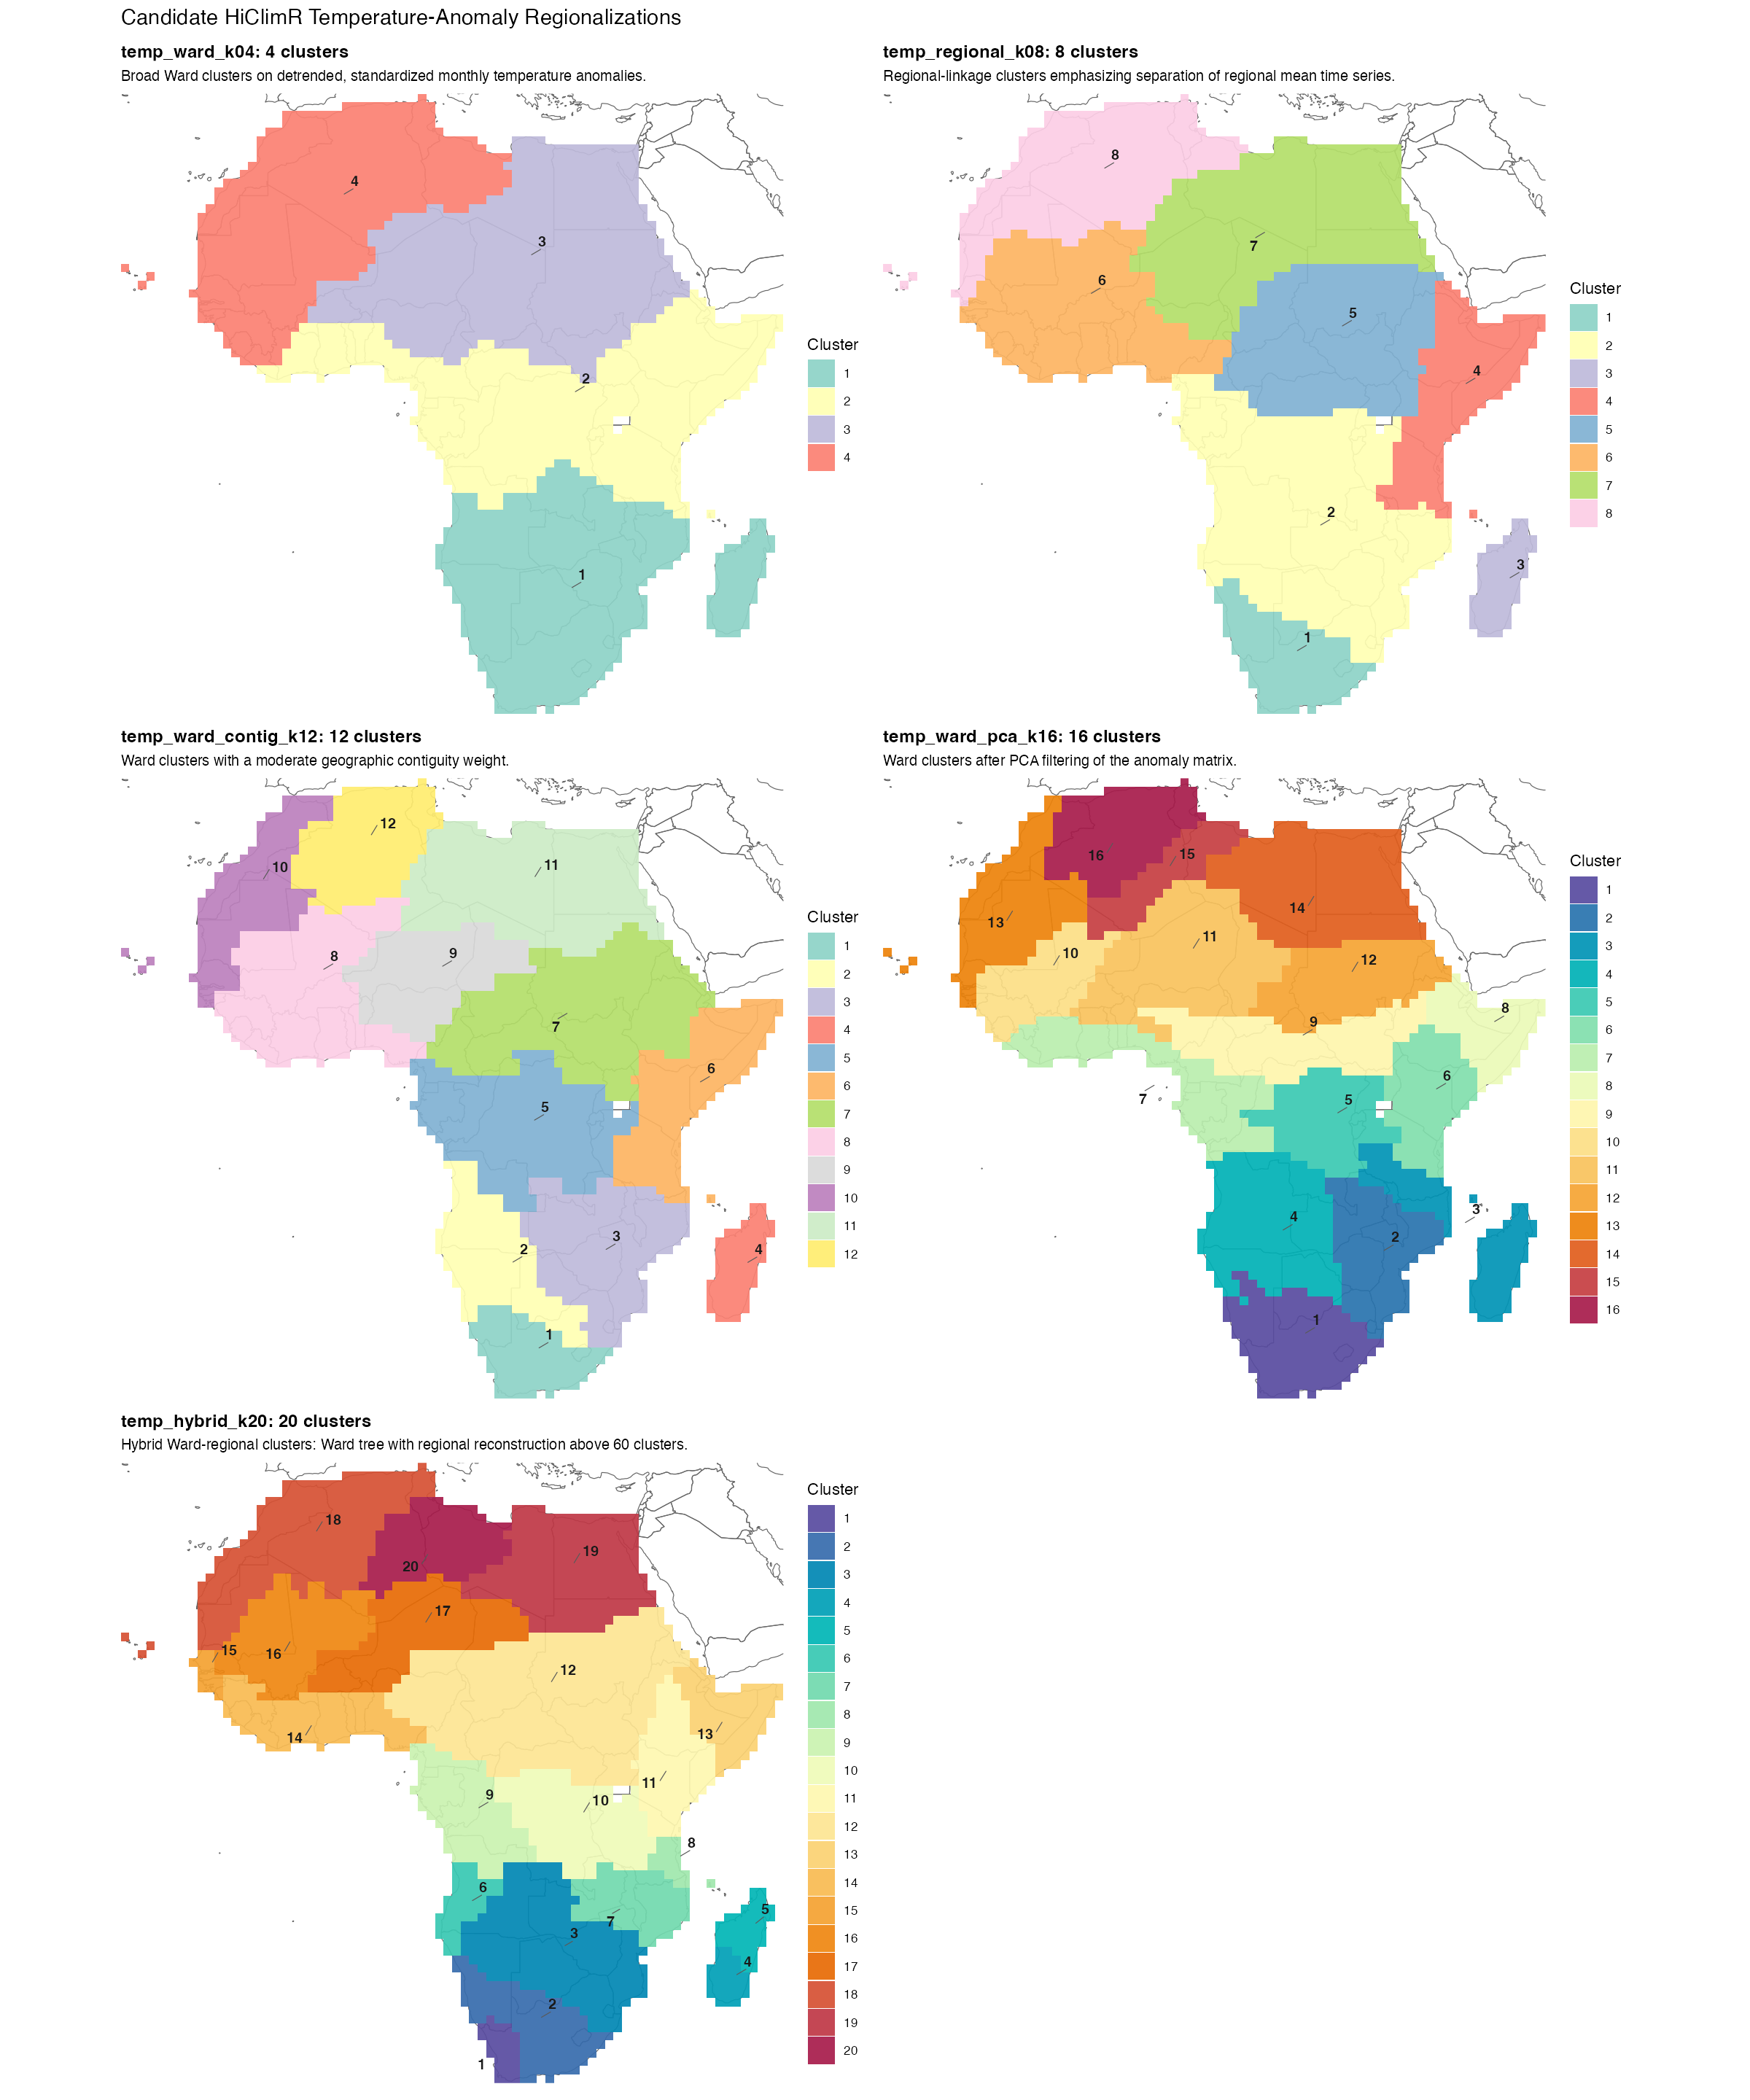
\includegraphics[width=0.92\linewidth,height=0.72\textheight,keepaspectratio]{all_clusterings_overview.png}
\caption{Candidate HiClimR partitions from \(G=4\) to \(G=20\). The figure shows the central trade-off: finer regionalizations add climate detail but produce smaller and less balanced inference groups.}
\label{fig:all-clusters}
\end{figure}

Moving from \(G=4\) to \(G=20\) adds climatic detail, but regions become
more fragmented and unequal. BCH does not reward more clusters
mechanically. The question is whether groups are large enough for
group-score normality and separated enough for weak cross-group
dependence. Figure \ref{fig:all-clusters} therefore frames the empirical
exercise as sensitivity over plausible, but not automatically valid,
climate partitions.

\%---------------------------------

\subsection{Implementation in R}

\%---------------------------------

The implementation separates estimation from inference. The
fixed-effects model is estimated once using monthly conflict incidence
as the outcome, monthly temperature anomaly as the treatment, grid-cell
fixed effects, and year-month fixed effects. The clustered covariance
matrix is then recomputed after assigning each grid cell to a candidate
climate region. For each grouping, scalar tests use \(G-1\) degrees of
freedom, matching the BCH fixed-\(G\) reference distribution up to small
finite-sample scaling.

The exact software command is reported in the replication code rather
than in the main text. This avoids making the essay read like a
programming manual while preserving reproducibility. For joint Wald
restrictions, BCH derive a scaled \(F\) reference; ordinary regression
summaries do not automatically impose that scaling.

\%---------------------------------

\subsection{Results}

\%---------------------------------

The point estimate does not depend on the inference group because the
regression is unchanged. The estimate is \[
\widehat\beta=0.00146.
\] Since \(Y_{it}\) is binary, this equals \(0.146\) percentage points.
Relative to the \(2.916\%\) baseline, it is about a \(5.0\%\) increase
for a \(1^\circ C\) positive anomaly. Uncertainty depends on \(G\).

\begin{table}[H]
\centering
\caption{Temperature anomaly and monthly conflict incidence with HiClimR-group inference}
\label{tab:bch-results}
\begin{tabular}{lrrrrr}
\toprule
Groups & \(\widehat\beta\) & SE & \(t\) & \(p\) & 95\% CI\\
\midrule
\(G=4\)  & 0.00146 & 0.00064 & 2.279 & 0.107 & [-0.00058, 0.00349]\\
\(G=8\)  & 0.00146 & 0.00046 & 3.152 & 0.016 & [ 0.00036, 0.00255]\\
\(G=12\) & 0.00146 & 0.00051 & 2.845 & 0.016 & [ 0.00033, 0.00258]\\
\(G=16\) & 0.00146 & 0.00050 & 2.919 & 0.011 & [ 0.00039, 0.00252]\\
\(G=20\) & 0.00146 & 0.00050 & 2.894 & 0.009 & [ 0.00040, 0.00251]\\
\bottomrule
\end{tabular}
\end{table}

The preferred interpretation emphasizes \(G=4\). It is the coarsest and
most balanced partition, so it best matches the BCH intuition. Under
this conservative partition, the 5 percent confidence interval includes
zero. Finer partitions give smaller \(p\)-values, but rely on smaller
and less regular groups. The \(G=20\) hybrid partition, for example, has
a group with only 14 cells. These rows are robustness checks, not the
main benchmark.

This is the central empirical result. The point estimate is stable
because grouping does not change the regression. Precision changes
because grouping changes the information used for inference. The
fixed-effects estimate is positive. Under the most conservative
grouping, it remains positive but imprecise.

Figure \ref{fig:app-var} connects the results table back to the
simulation. The table reports coefficient inference; the figure shows
the variance object behind it. The purpose is not to select the \(G\)
with the lowest variance, but to show how uncertainty changes when the
same score is aggregated into different climate groups.

\begin{figure}[H]
\centering
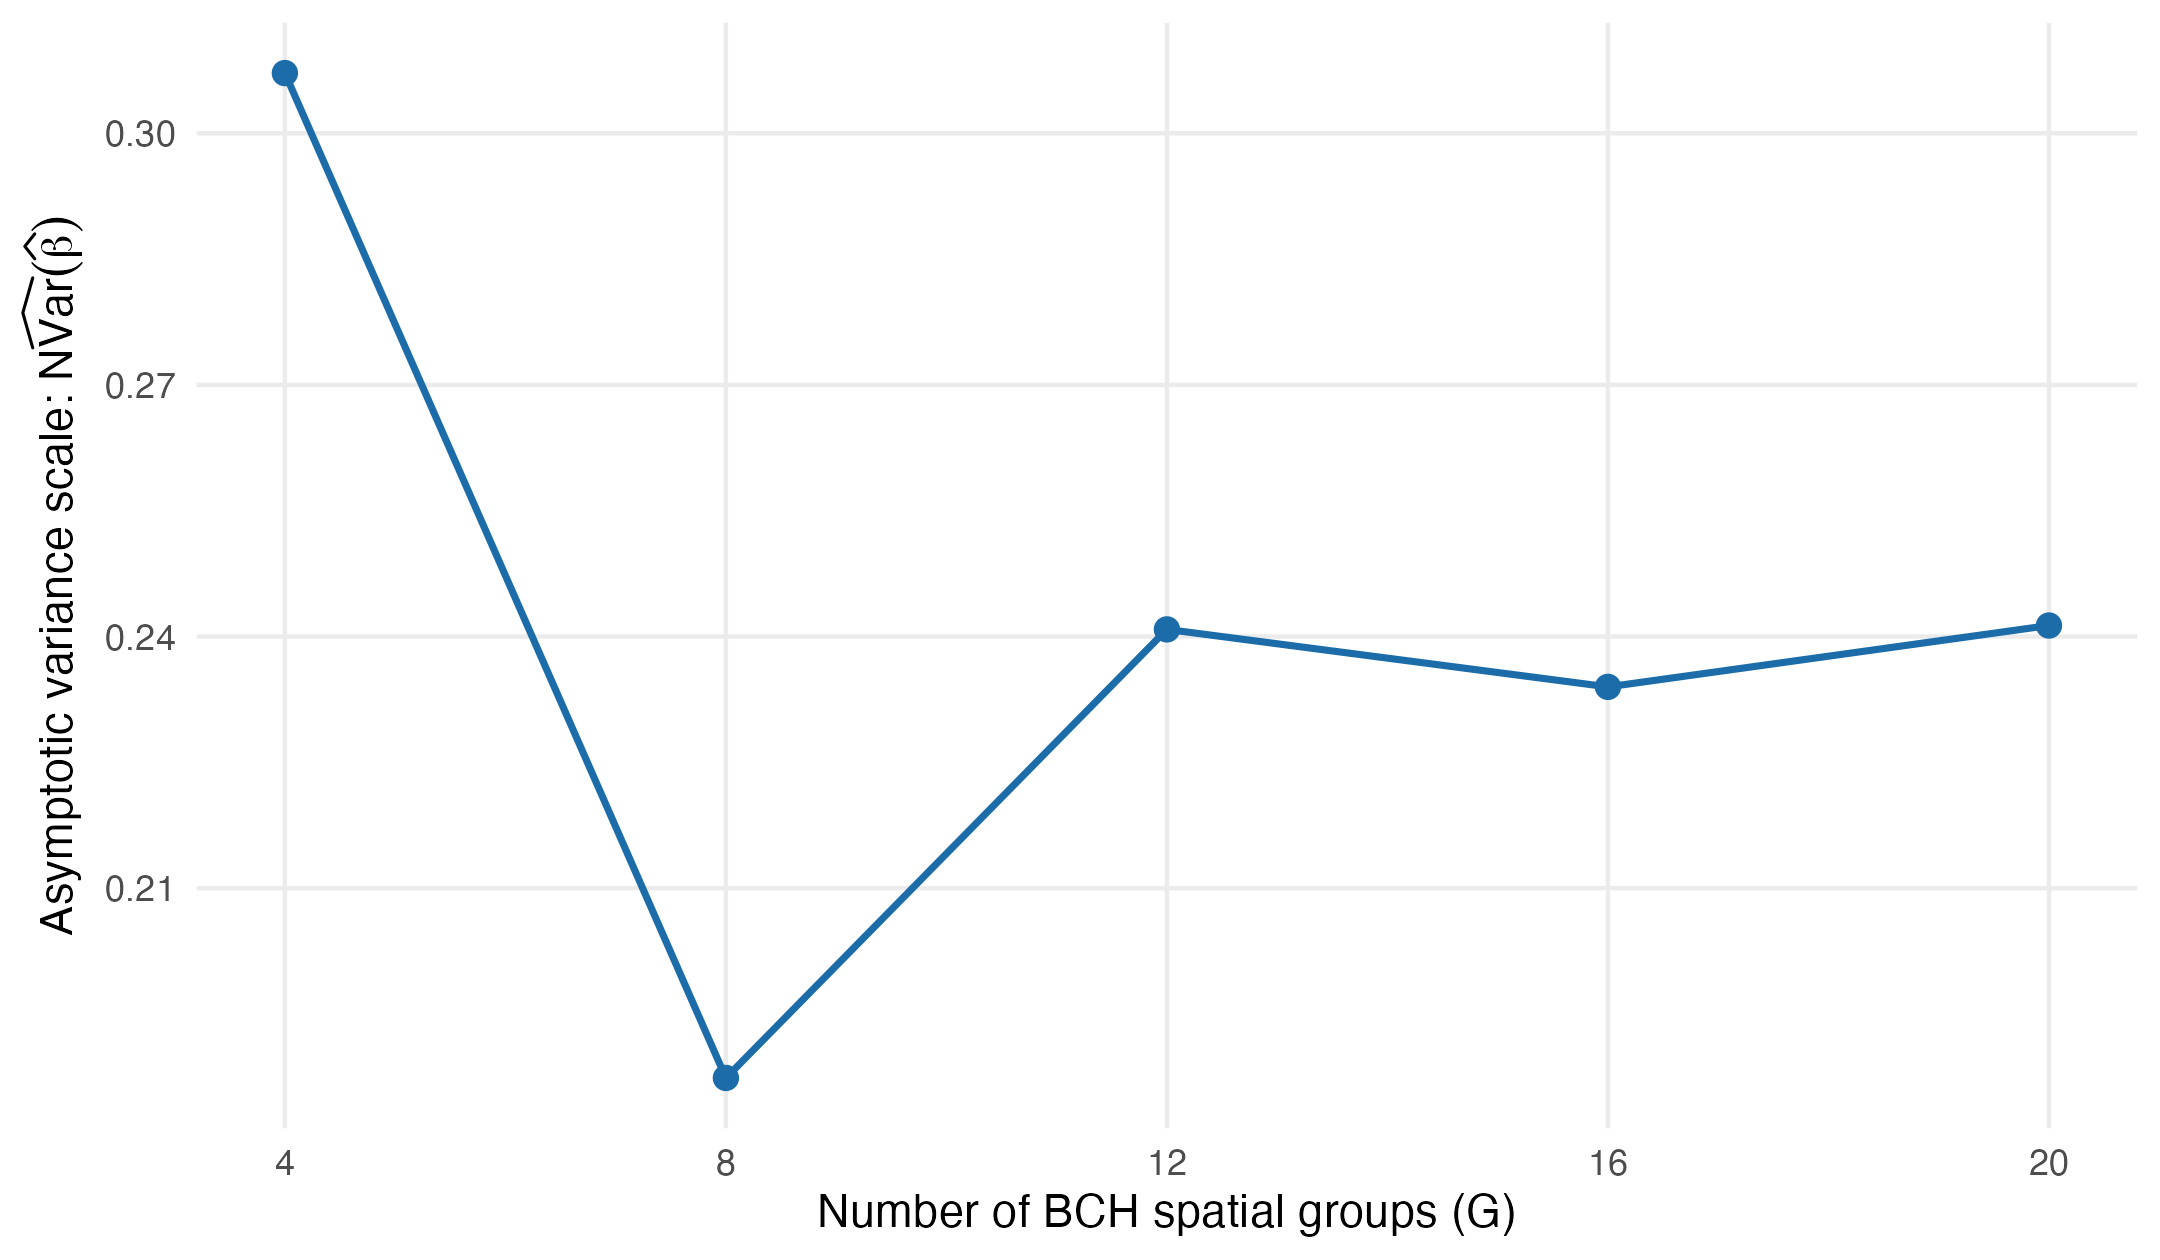
\includegraphics[width=0.56\linewidth]{bch_application_variance_by_g.png}
\caption{Sensitivity of the asymptotic-scale variance estimate to the number of BCH groups. The non-monotonic pattern is expected: changing \(G\) changes both group score aggregation and the finite-\(G\) reference distribution.}
\label{fig:app-var}
\end{figure}

Figure \ref{fig:app-var} sharpens the main empirical lesson. The
variance estimate is not a smooth decreasing function of \(G\). Changing
\(G\) changes score aggregation and scalar-test degrees of freedom. The
\(G=4\) result is cautious because it treats independent information as
four large climate regions. Finer partitions make the positive estimate
more precise, but that precision is persuasive only if score diagnostics
support the implied cross-group independence.

\%---------------------------------

\subsection{Score Diagnostics and an Administrative Benchmark}

\%---------------------------------

A defensible BCH application must check whether groups produce
approximately independent scores. This is where the data-driven
construction can be compared to administrative benchmarks. We use two:
five AU-style macroregions and 51 country/territory groups. For the
scalar temperature coefficient, let \(x_{it}=A_{it}\) after
residualizing on fixed effects. The monthly score contribution is
approximately \[
s_{it}=x_{it}\widehat e_{it}.
\] For each group \(g\) and month \(t\), compute \[
S_{gt}=\sum_{i\in g}s_{it}.
\] The diagnostic object is the \(G\times G\) correlation matrix of
\(S_{gt}\) over time. A good grouping has low off-diagonal correlations.
No single group should dominate the variance. No obvious neighbor-pair
dependence should remain. This is stricter than testing temperature
homogeneity.

\begin{table}[H]
\centering
\caption{Score-independence diagnostics by grouping rule}
\label{tab:score-diagnostics}
\scriptsize
\begin{tabular}{lrrrrr}
\toprule
Grouping rule & \(G\) & Cell size min/med/max & Mean \(|\rho|\) & Max \(|\rho|\) & BCH \(p\)\\
\midrule
HiClimR \(G=4\)  & 4  & 618/670/738 & 0.101 & 0.192 & 0.107\\
HiClimR \(G=8\)  & 8  & 66/369/636  & 0.088 & 0.349 & 0.016\\
HiClimR \(G=12\) & 12 & 66/196/396  & 0.093 & 0.353 & 0.016\\
HiClimR \(G=16\) & 16 & 90/168/279  & 0.083 & 0.348 & 0.011\\
HiClimR \(G=20\) & 20 & 14/124/472  & 0.079 & 0.621 & 0.009\\
Admin macroregions & 5 & 435/446/822 & 0.114 & 0.232 & 0.076\\
Countries        & 51 & 1/33/219     & 0.076 & 0.864 & 0.012\\
\bottomrule
\end{tabular}
\end{table}

Table \ref{tab:score-diagnostics} is mixed but useful. Mean absolute
score correlations are modest for all rules, so averages alone do not
choose the grouping. The maxima and group sizes are more revealing.
HiClimR \(G=4\) and administrative macroregions both use a small number
of large groups and produce cautious inference. HiClimR \(G=4\) has the
lower maximum score correlation, \(0.192\) versus \(0.232\), because its
boundaries follow climate co-movement rather than inherited regional
classifications. Countries provide many degrees of freedom, but include
one-cell units and a maximum score correlation of \(0.864\). They are
familiar clusters, not automatically valid BCH groups.

The diagnostic supports a conservative ranking. Data-driven climate
groups are not valid because an algorithm produced them. They are
relevant because they are chosen from treatment dynamics and then
evaluated on regression scores. The central comparison is therefore
\(G=4\) HiClimR versus administrative macroregions. Both answer the
small-entity correlation problem with few large groups. The climate
grouping performs at least as well on score independence and is directly
tied to the weather process. Finer HiClimR partitions and country
clusters are robustness checks, not automatic improvements.

\%=================================

\section{Conclusion}

\%=================================

The BCH lesson is that clustered inference is not a mechanical search
for many clusters. In spatial panels, a few large, well-shaped groups
may be more credible than many fine units. The simulation shows why.
With fixed \(G\), the variance estimator remains random, and \(t_{G-1}\)
critical values are the natural scalar reference.

The application gives a reproducible workflow. HiClimR defines climate
regions from temperature-anomaly co-movement. A fixed-effects regression
estimates the relationship between monthly temperature anomalies and
monthly conflict incidence. Inference is clustered by the chosen climate
group. Score diagnostics then ask whether group sums are close to
independent. The temperature-conflict association is positive and
modest. Its precision depends on the maintained group structure. The
most defensible \(G=4\) partition gives cautious evidence, not a
decisive rejection of no effect.

The administrative benchmarks clarify what the data-driven approach
adds. Macroregions are a credible geographer-style alternative and lead
to the same cautious conclusion as HiClimR \(G=4\). Country borders
offer many degrees of freedom, but include one-cell units and a very
high maximum score correlation. HiClimR does not validate BCH inference
by itself. It makes the grouping rule explicit, tied to climate
exposure, and testable at the score level.

The final conclusion is therefore conservative. The number of groups
matters because it changes both the covariance estimate and the
finite-\(G\) reference distribution. Group choice matters because formal
degrees of freedom are useful only if the corresponding group scores are
close to independent. In this application, the positive
temperature-conflict association is robust in sign but not in
inferential strength. That is exactly the type of distinction
fixed-\(G\) inference is designed to make visible.

\bibliography{references.bib}

\end{document}
